%Dernières modifications E. Rouquette (12/2023)

%%%%%%%%%%%%%%%%%%%%%% PRÉAMBULE


%%%%%%%%%%%%%% partie obligatoire du préambule
\documentclass[a4paper,12pt,twoside]{book}
\usepackage{fontspec}
\usepackage{xunicode}
\usepackage[french]{babel}%on peut préciser d'autres langues.


%%%%%%%%%%%%%%%%%%%%%%%%%%%%%%%%% PACKAGES UTILISÉS

\usepackage{csquotes} % les guillemets français
\usepackage{lettrine} %faire une lettrine (pas obligatoire)

\usepackage[backend=biber,style=enc,sorting=nyt,maxbibnames=10]{biblatex}%charger le style de l'EnC (téléchargeable ici https://ctan.org/pkg/biblatex-enc)
\addbibresource{./bibliographie.bib} %le fichier bibliograhique. Exemple de chemin à partir du dossier où se trouve le document maître:Exemple ./dossierA/fichier.bib
%\defbibheading{}{\subsection*{}} Si l'on veut changer le titre de la/les bibliographie(s)


%%%Faire un ou plusieurs index

%\usepackage{imakeidx} %pour faire un ou plusieurs index
%\makeindex %commande pour générer l'index


%RAJOUTEZ ICI VOS PACKAGES
\usepackage{longtable} % Pour les longs tableaux
\usepackage{array}     % Pour une meilleure mise en forme des colonnes



%%%%%%%%%%%%%%%%%%%%%%%%%%%%%%%%% CONFIGURATION DE MISE EN PAGE

%%%%%% Les compteurs (sections, subsections, etc)


%%%%%% Les compteurs (sections, subsections, etc)
\renewcommand{\thesection}{\Roman{section}.}%On ne fait apparaître que le numéro de la section
\renewcommand{\thesubsection}{\arabic{subsection}.}%subsection en chiffres arabes
\renewcommand{\thesubsubsection}{\alph{subsubsection}.}%subsubsection en lettres minuscules
%Si l'on veut faire apparaître les subsubsection dans le table des matières (à commenter sinon)
\setcounter{tocdepth}{3}
\setcounter{secnumdepth}{3}  % La subsubsection (profondeur=3 dans la table des matières) apparait numérotée dans la TdM



%%%%%  Configurer le document selon les normes de l'école

\usepackage[margin=2.5cm]{geometry} %marges
\usepackage{setspace} % espacement qui permet ensuite de définir un interligne
\onehalfspacing % interligne de 1.5
\setlength\parindent{1cm} % indentation des paragraphes à 1 cm

%%%%% Mise en forme des headers (haut de page)

\usepackage{fancyhdr} %package utilisé pour modifier les headers
\pagestyle{fancy} %utiliser ses propres choix de mise en page et non ceux par défaut du package

\setlength\headheight{16pt}%la hauteur des headers
\renewcommand{\sectionmark}[1]{\markright{\small\textit{\thesection~\  #1}}}%Faire apparaître dans les headers les sections en  petit et en italiques
\renewcommand{\sectionmark}[1]{}%Commenter la lign précédetne et mettre celle-ci pour ne pas avoir le titre des sections dans le header
\renewcommand{\chaptermark}[1]{\markboth{\small\chaptername~\thechapter~--\ \textit{#1}}{}}%idem pour les chapitres
%\renewcommand{\chaptermark}[1]{}%Commenter la ligne précédente et mettre celle-ci pour ne pas avoir le titre des chapitres  dans le header



%indiquer des règles d'hyphénation pour des mots précis si besoin
%\begin{hyphenrules}{french}
%	\hyphenation{}
%\end{hyphenrules}


%%%%%%% Package hyperref
% A mettre après les autres appels de packages car redéfinit certaines commandes).

\usepackage[colorlinks=false, breaklinks=true, pdfusetitle, pdfsubject ={Mémoire HN}, pdfkeywords={les mots-clés}]{hyperref} %
\usepackage[numbered]{bookmark}%va avec hyperref; marche mieux pour les signets. l'option numbered: les signets dans le pdf sont numérotés

% Compléter pdfsubjet et pdfkeywords
%Explication des options de hyperref (modifiables)
% hyperindex=false
% colorlinks=false: pour que le cadre des liens n'apparaisse pas à l'impression
% breaklinks permet d'avoir des liens allant sur pusieurs lignes
%pdfusetitle: utiliser \author et \title pour produire le nom et le titre du pdf






%%%%%%%%%%%%%%%%%%%% Package glossaries

%Exception: il faut le charger APRÈS hyperref
\usepackage[toc=true]{glossaries}
\makeglossaries
%avec TexStudio: F9 pour compiler le glossaire (s'il y a aussi un index)
\loadglsentries{./glossaire.tex}

%Structure d'une entrée de glossaire
%\newglossaryentry{}{%
%	name={},%
%	description={}
%}



%%%%%%%%%%%%%%%%%% DÉFINITION DES COMMANDES ET ENVIRONNMENTS







 %%%%%%%%%%%%%% INFORMATIONS POUR LA PAGE DE TITRE
\author{Anna Le Duff- M2 TNAH}
\title{Normaliser les données culturelles pour optimiser leur circulation :  l'utilisation du modèle LIDO.
}

%%%%%%%%%%%%%%%%%%%%%% DOCUMENT
\begin{document}
	\begin{titlepage}
		\begin{center}
			
			\bigskip
			
			\begin{large}				
				ÉCOLE NATIONALE DES CHARTES\\
				UNIVERSITÉ PARIS, SCIENCES \& LETTRES
			\end{large}
			\begin{center}\rule{2cm}{0.02cm}\end{center}
			
			\bigskip
			\bigskip
			\bigskip
			\begin{Large}
				\textbf{Anna Le Duff}\\
			\end{Large}
		%selon le cas
			\begin{normalsize} \textit{licencié.e ès lettres}\\

			\end{normalsize}
			
			\bigskip
			\bigskip
			\bigskip
			
			\begin{Huge}
				\textbf{Normaliser les données culturelles pour optimiser leur circulation : }\\
			\end{Huge}
			\bigskip
			\bigskip
			\begin{LARGE}
				\textbf{L'utilisation du modèle LIDO.}\\
			\end{LARGE}
			
			\bigskip
			\bigskip
			\bigskip
			\begin{large}
			\end{large}
			\vfill
			
			\begin{large}
				Mémoire 
				pour le diplôme de master \\
				\enquote{Technologies numériques appliquées à l'histoire} \\
				\bigskip
				2024
			\end{large}
			
		\end{center}
	\end{titlepage}

	\thispagestyle{empty}	
	\cleardoublepage
	
\frontmatter

	\chapter{Résumé}
\medskip
        \textbf{Résumé en français :}
Ce mémoire explore la normalisation des données culturelles, avec un focus particulier sur l'utilisation du modèle LIDO (Lightweight Information Describing Objects) en temps que modèle de circulation de données pour l'agrégation des informations muséales par le Ministère de la Culture. Dans un contexte où les institutions culturelles font face à une fragmentation des données, le travail examine comment standardiser ces informations pour les rendre interopérables et exploitables à des fins de recherche, de diffusion ou de réutilisation. Le projet met en lumière les défis techniques liés à l'hétérogénéité des formats et des systèmes utilisés, ainsi que l'importance de l'agrégation à l'échelle nationale et européenne. \newline

\textbf{Résumé en anglais :}
This thesis explores the standardization of cultural data, with a particular focus on the use of the LIDO model (Lightweight Information Describing Objects) as a data circulation model for the aggregation of museum information by the Ministry of Culture. In a context where cultural institutions face data fragmentation, the work examines how to standardize this information to make it interoperable and usable for research, dissemination, or reuse. The project highlights the technical challenges related to the heterogeneity of formats and systems used, as well as the importance of aggregation at both national and European levels. \newline
	
	\textbf{Mots-clés:} Normalisation des données~; Interopérabilité~; Modèle LIDO~; Agrégation culturelle.\newline

	\textbf{Informations bibliographiques:} Anna Le Duff, \textit{Normaliser les données culturelles pour optimiser leur circulation :  l'utilisation du modèle LIDO.}, mémoire de master \enquote{Technologies numériques appliquées à l'histoire}, dir. [Axel Roche Dioré], École nationale des chartes, 2024.

		\newpage{\pagestyle{empty}\cleardoublepage}
	
	\chapter{Remerciements}
	
\lettrine{M}es remerciements vont tout d'abord à Marie Véronique Leroi et Thierry Bultingaire, sous la
responsabilité de qui j’ai eu la chance d’effectuer mon stage au sein du Service du numérique du Ministère de la Culture. Merci pour leurs encouragements, leur bienveillance et leur confiance, qu'ils m'ont donné tout au long du stage mais aussi pendant la rédaction de ce mémoire. \newline

Je tiens également à remercier toute l'équipe du DPNC, qui ont fait de mon stage une expérience inoubliable. Ainsi que Antoine Courtin et Gautier Poupeau, pour tout nos échanges.\newline

Mes remerciements à Axel Roche-Dioré, mon tuteur pour ce
mémoire, pour tout ses conseils.\newline

Enfin, je remercie chaudement Mélina et Claire, pour leur relecture et leurs encouragements pendant les derniers jours.
	\newpage{\pagestyle{empty}\cleardoublepage}
	
%%%%%%%%%%%% \bibliographie ici (normes de l'EnC)
\printbibliography
	
\chapter{Introduction}	
\begin{quote}
    “ Les musées, gardiens et interprètes des témoignages initiaux de nos civilisations, seront les dépositaires des informations primaires qui devront être saisies et représentées sous de nouvelles formes. Leur rôle sera d'expliquer, d'explorer et d'élargir l'univers dans un nouveau langage multimédia. [...] Pour mener à bien cette mission, les gardiens de notre patrimoine vont devoir entreprendre dès maintenant les tâches suivantes : a) superviser le traitement numérique des informations  concernant ce patrimoine selon des normes garantissant la valeur de leur investissement ; 6) définir une politique de délivrance de licences protégeant l'utilisation des informations créées ; enfin c) explorer les possibilités de coopération  et de mise en commun  de l'information, sachant que les mondes culturel et social auxquels les collections sont associées peuvent être représentés selon les catégories courantes de la connaissance. La première tâche exige des responsables des musées  qu'ils entreprennent la saisie et l'informatisation des données qui se rapportent à leurs collections et à l'environnement auquel elles se réfèrent ; qu'en même temps ils constituent un fonds d'archives sonores et vidéo sur leurs collections en formats numériques  normalisés. Le Comité pour les échanges d'informations informatisées entre les musées (CIMI) a estimé que le meilleur moyen de préserver durablement ces données est de les indexer en utilisant le langage standard généralisé de balisage (SGML) (IS0 8879) et les mêmes modèles logiques de classement des données. Les systèmes informatiques contribuant à cette nouvelle documentation des collections doivent  être pleinement accordés à l'ensemble des activités du musée, de l'acquisition à l'exposition, et tenir compte des politiques et des procédures propres à chaque institution plutôt  que d'être greffés sur la  programmation existante et considérée comme une activité supplémentaire. 
[...]
Demain, des musées automatisés de ces données seront contraints de négocier avec  des centaines de musées. A l'heure actuelle, la  législation relative au traitement des droits sur les données numériques et au patrimoine culturel varie considérablement d'un pays à l'autre : c'est pourquoi, dans chaque pays, les musées doivent élaborer en commun des mécanismes de gestion de leurs droits dans ce domaine. Ils doivent également s'associer pour assurer la diffusion de ces matériels à l'extérieur de l'institution, sous peine de les voir tomber très vite dans le domaine public en vertu de la loi ou de l'usage [...] Surtout, l'institution  aurait perdu une occasion unique  d'ouvrir une brèche par laquelle les collections vont pouvoir envahir les maisons, les écoles, la rue, les lieux de travail. Dans cet espace, les interprétations et représentations des collections des musées vont devenir un instrument irremplaçable de sensibilisation du public à la culture et à la nature. Il reviendra aux musées du XXI siècle d'explorer ces possibilités, de proposer des expériences associant représentations abstraites et objets concrets dans une vision neuve, complexe, culturellement structurée et authentique du monde.”\footcite{Bearman_1994}
\end{quote} 
La question de la gestion des données culturelles s’est posée dès lors que les institutions se sont dotées de systèmes informatiques. Pour David Bearman, rédacteur en chef de la revue trimestrielle \textit{Archives and Museum Informatics}, les choses sont claires. Dans son article publié dans \textit{Museum International} en 1994, celui-ci décrit déjà les différentes étapes qu’il faudrait suivre pour garantir la qualité des données produites par les institutions culturelles et pour pouvoir les exploiter au mieux. Lors de la lecture de cet article, nous nous sommes immédiatement rendu compte que les règles évoquées faisaient encore partie de la réflexion aujourd'hui 30 ans plus tard. Parmi les règles qu’il évoque, la première règle est celle de la normalisation, la troisième est celle de la réflexion sur la mise en commun de ces données. \newline

Lors de notre stage au sein Service du numérique du ministère de la culture (SNUM), ces deux règles et donc éléments de réflexions ont été au centre de notre travail. 
L’objectif de notre stage à été de s’assurer que le modèle LIDO (Lightweight Information Describing Objects ) était un modèle de données conforme aux besoins très hétérogènes des partenaires culturels du ministère de la culture. Le modèle en question, que nous définirons plus en détail plus tard dans ce mémoire, est un schéma de données XML dérivé du CIDOC CRM (CIDOC Conceptual Reference Model), utilisé pour décrire et échanger  des collections muséales. Le modèle LIDO est celui qui va être utilisé pour servir de modèle d'échange de données entre les institutions et le ministère de la Culture. Les thèmes de la normalisation et de la mise en commun de l’information nous ont donc accompagné au long de notre projet. \newline

La mission du stage s’inscrit dans le cadre de la stratégie nationale d’agrégation des contenus culturels portée par le ministère de la Culture et sa mise en oeuvre:
L’agrégation des contenus culturels est un processus qui permet la collecte des liens vers les images et des métadonnées descriptives des œuvres détenues par des institutions culturelles. L’objectif est leur diffusion sur des portails, thématiques, régionaux, nationaux (comme par exemple la plateforme ouverte du patrimoine POP pour les données réglementaires autour des collections des Musées de France ou les données du patrimoine ou de l’inventaire) ou encore européens. C’est le cas d’Europeana \footcite{europeana}, un portail qui se propose de donner accès à plusieurs millions de contenus numérisés provenant d’institutions culturelles de toute l’Europe. Mais aussi, dans le futur, l’espace données culturel européen. Les espaces de données européens sont le produit de la stratégie data de la Commission européenne, pour rendre plus de données disponibles à la consultation et surtout à la réutilisation. Quatorze espaces de données européens sont en cours de spécification et de déploiement, chacun portant sur un domaine d'intérêt public, comme la santé, l’énergie ou les finances\footcite{eecd}.\newline

Le but du ministère, en collectant ces données culturelles, est d'offrir un point d’accès unique à une masse de contenus découvrables, pour faciliter une visibilité à toutes les échelles du patrimoine conservé par les institutions culturelles. 
L’agrégation devrait également permettre de rendre les données culturelles disponibles pour différentes réutilisations par d’autres acteurs que le milieu culturel, par exemple pour l’enseignement, la recherche ou encore le tourisme.
Le ministère de la Culture a pour mission d’agréger les données culturelles (notamment muséales et patrimoniales) de l’ensemble du territoire français, ne relevant pas du champ des données bibliographiques (livre, périodiques et imprimés qui sont pris en charge par l’agrégateur Gallica géré par la Bibliothèque Nationale de France) et des archives (prises en charge par l’agrégateur FranceArchives géré par le Service Interministériel des Archives de France).\newline 

Dans le cadre de cette mission, le ministère fait face à une grande diversité de formats et de protocoles utilisés par les différents établissements culturels. 
Cette diversité de pratiques a conduit à une fragmentation des données, chaque établissement développant ses propres méthodes de gestion de données en fonction de ses besoins spécifiques. Le terme de fragmentation des données définit un phénomène lors duquel les données sont dispersées et sont parfois trop différentes pour pouvoir les faire communiquer entre elles. 
C’est d’autant plus vrai que les établissements culturels font, pour la plupart, appel à des éditeurs de logiciels pour développer des solutions de gestion de collections ainsi que d'édition de leurs données. Ces éditeurs proposant chacun des solutions différentes et développant des outils de marché, cela participe à la fragmentation des données. Le paradoxe étant que beaucoup d'institutions sont très satisfaites de ce système car il leur permet d’accéder à des solutions personnalisées, répondant donc à leurs besoins principaux : ceux de la gestion en interne.\newline

Pendant de nombreuses années le ministère était organisé en silos avec une base/application par type de données, ce qui limitait la possibilité d'une approche transversale de la gestion des collections. Chaque proposition (applications ou autres) faite par le service, était développée pour répondre aux besoins spécifiques de chaque établissement, sans véritable souci de compatibilité ou d'interopérabilité \footnote{\emph{Interopérabilité }: Informatique
Capacité de matériels, de logiciels ou de protocoles différents à fonctionner ensemble et à partager des informations : Interopérabilité des réseaux téléphoniques. Source : Dictionnaire Larousse en ligne”}avec d'autres systèmes. La réorganisation et la création du Service du Numérique (SNUM) a remis à plat cette organisation et vise donc à casser ces silos et permettre l’interopérabilité des données tout en préservant les spécificités des différents métiers. L'objectif est de proposer une approche plus unie et une direction commune, permettant non seulement de rationaliser la collecte des données, mais aussi de standardiser les formats pour faciliter leur utilisation à des fins de recherche, de circulation, d'exposition ou d'exploitation par d'autres acteurs culturels.\newline 

C’est dans ce contexte de pratiques diverses que le besoin de normalisation des données s’est posé. En effet pour pouvoir mener à bien cette mission d'agrégation il faut réfléchir à un modèle de données qui soit commun aux données collectées pour permettre leurs circulation et ainsi exploitation. 
La normalisation est un processus essentiel pour transformer des informations hétérogènes en données homogènes, interopérables et exploitables. Cela s'inscrit dans une longue tradition de gestion de l'information dans les institutions culturelles, ainsi que dans tous les domaines qui ont besoin d’exploiter des données, quelles qu’elles soient. 
Depuis les premiers catalogues et livres d'inventaires jusqu'aux systèmes de classification modernes, la question de l'uniformisation des données a été un enjeu crucial. Normaliser, c'est avant tout rendre les données comparables, facilitant ainsi la recherche et l'interopérabilité entre les différents systèmes. \newline


Ce mémoire se propose donc d'explorer l'histoire et les enjeux de la normalisation des données culturelles, en s'intéressant particulièrement à son application dans le contexte des musées. Si les bibliothèques et les archives ont été pionnières en matière de normalisation, les musées ont longtemps accusé un certain retard. Aujourd'hui, cependant, ces institutions commencent à atteindre une certaine maturité dans ce domaine, notamment grâce à l'émergence d’initiatives de grande envergure, comme celle de l'agrégation des données muséales à l'échelle nationale. Parmi ces initiative sil nous faut mentionner l’harmonisation des données de la base Joconde, qui est le catalogue collectif des collections des musées de France. \newline Nous explorerons par la suite les standards et sytèmes de gestion de données utilisés aujourd'hui dans les muséee.\newline Pour finir, nous expliquerons comment nous avons vérifié que le modèle LIDO corresponde bien aux besoins de de normalisation essentiels pour mener à bien notre objectif d’agrégation des données culturelles françaises.

\begin{figure}[h!]
	\centerline{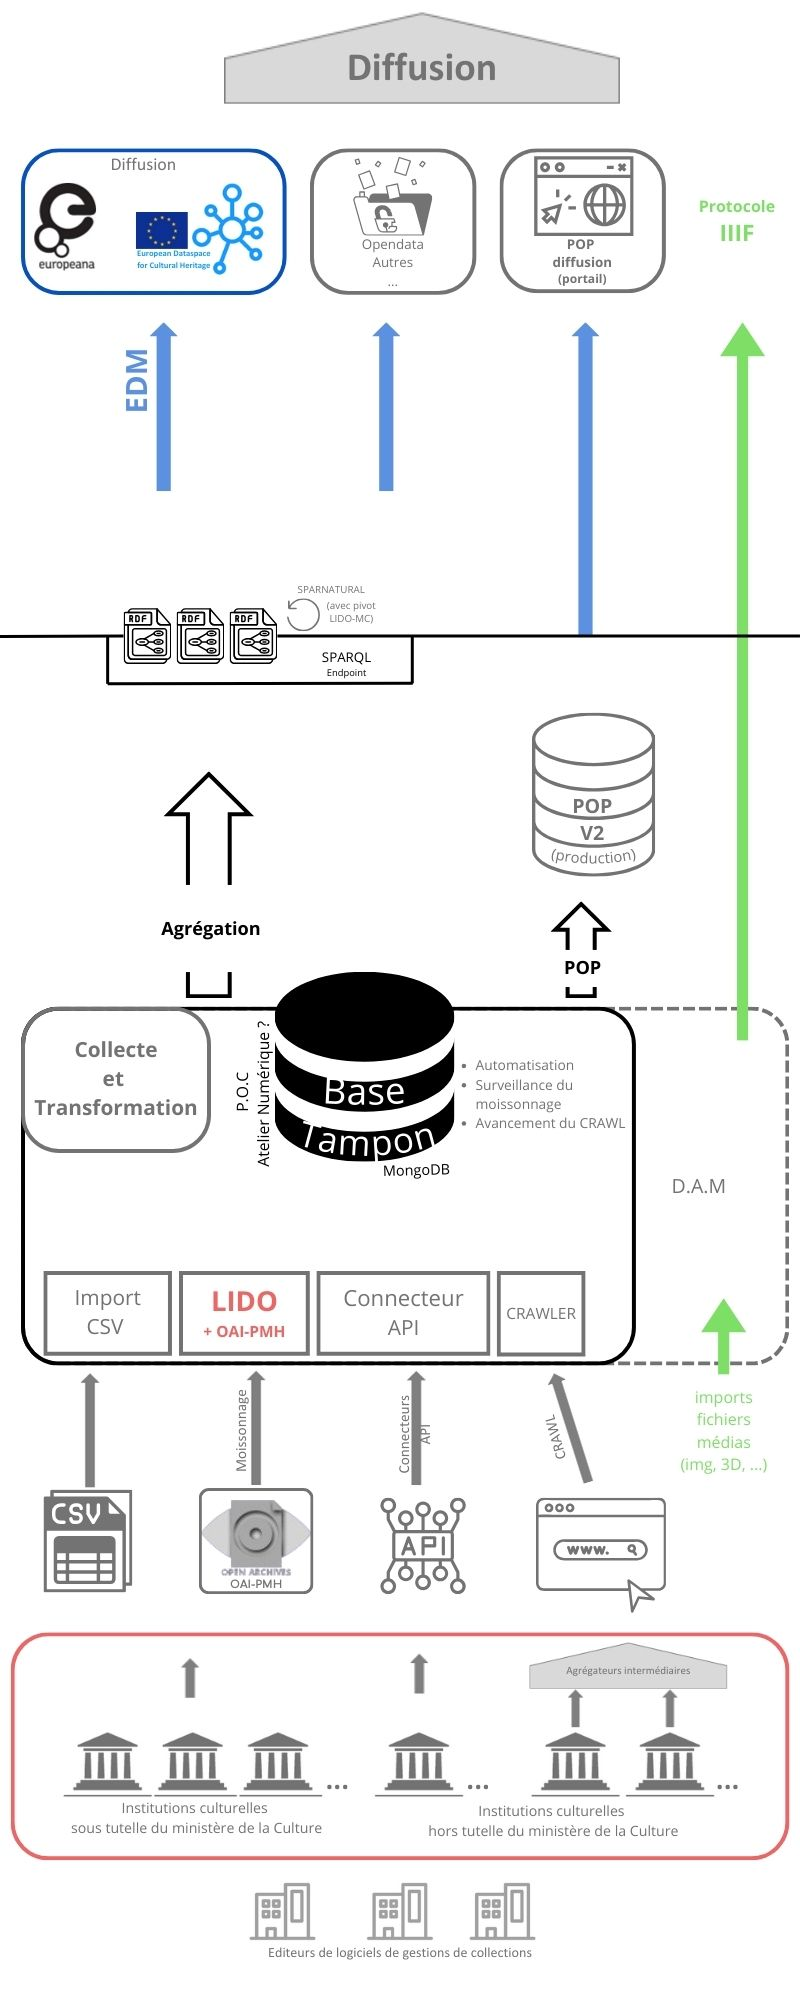
\includegraphics [height=0.8\textheight]{medias/schema_agregation.jpg} }
	\caption{Schéma illustrant la stratégie d'agrégation du Ministère de la Culture}
\end{figure}
\newpage{\pagestyle{empty}\cleardoublepage}

%%%%%%%%%%%%%%%%%Le corps du mémoire
	\mainmatter
%Trier par dossiers si besoin (front, main,annexes,), se crérer un docuemnt .tex par structure (section ou chapter selon la taille et la pertinence) Exemple de chemin à partir du dossier où se trouve le document maître: ./dossierA/fichier.tex

	

	\part{Histoire et enjeux de la normalisation des données culturelles}
\textbf{Une brève introduction aux concepts.}\newline

L’enjeux principal que nous avons rencontré lors de notre stage à été celui de la normalisation des données pour répondre aux besoins de l’agrégation.  \newline

Comme décrit plus tôt, la normalisation, en général, est un processus qui consiste à établir des critères ou des standards pour rendre les données homogènes, interopérables et facilement exploitables. En effet, se baser sur des critères communs permet ensuite à l’utilisateur de faire des comparaisons entre les données, de savoir les rechercher, et donc de pouvoir accéder à l’information. Dans le contexte des collections culturelles, ce processus revêt une importance cruciale, car il permet de structurer des données souvent disparates, collectées sous diverses formes, et de les rendre accessibles à travers des systèmes d’information interconnectés. \newline

Il faut noter que les données disparates sont le reflet des collections qu’elles représentent. Les collections culturelles, notamment celles conservées dans les musées peuvent être extrêmement variées, allant d’objets de beaux arts plus “classiques”, à des objets plus inhabituels, au sein de collections ethnographiques par exemple. 
Au-delà des objets divers qui peuvent être conservés, et donc mis en données, les données culturelles concernent aussi la vie de l’objet dans sa création: des dates, des titres (parfois plusieurs), des noms, des lieux etc… mais aussi la vie de l’objet dans les collections, avec des numéros d’inventaire, un historique d'appartenance, des données relevant de ses conditions de conservation, etc… \newline

Avant de parler plus en profondeur de la normalisation nous allons préciser au mieux la notion de “donnée”. En effet, celle-ci est au centre de toutes nos réflexions, mais il nous est difficile de lui trouver une définition qui représente toute sa complexité.
Dans son ouvrage \textit{Qu’est-ce que le travail scientifique des données ?}, Christine L. Borgman, convient elle-même que \begin{quote}
    <<Malgré ses cinq siècles d’existence, le terme data ou « donnée » n’a toujours pas trouvé une définition consensuelle.” Mais elle ajoute que “La synthèse la plus exhaustive consiste à dire que les données sont des représentations d’observations, d’objets ou d’autres entités qui servent à mettre en évidence des phénomènes à des fins de recherche.>> \footcite{borman_2020}
\end{quote}
La donnée est donc la représentation d’une certaine réalité à partir de laquelle on peut extraire un sens et des connaissances.

\chapter{La normalisation des données.}
\subsection{Historique de la normalisation, l’évolution des pratiques dans les bibliothèques et les archives.}

Avant d’aborder le sujet de la normalisation à grande échelle dans les musées, nous allons nous pencher sur l’historique de ce processus dans d'autres domaines culturels qui ont réfléchi à ces questions plus tôt . \newline

Comme nous l’avons évoqué précédemment, les bibliothèques et les archives ont été plus rapides dans l’adoption de ce processus. Au fil des décennies, bibliothèques, archives et musées ont accumulé d’énormes quantités de données, allant des descriptions physiques des objets aux informations contextuelles, telles que l’histoire des œuvres, leur créateur, leur signification culturelle, et les informations sur leur conservation. Ces instutions traitent souvent des fonds ou des documents faisant partie d'ensembles, pour s'y retrouver au sein de ceux-ci, les bibliothécaires on développé des outils. À l’origine, ces données étaient consignées sous forme de registres papier, catalogues ou inventaires. Ces systèmes fragmentés étaient destinés aux gestionnaires des collections, conservateurs et régisseurs par exemple. Ils étaient inaccessibles au grand public. \newline

La volonté de partage de l’information prend forme très tôt dans le domaine des bibliothèques. En effet, dès la Révolution française, on prend conscience q u'elles sont un axe central pour répondre au besoin d’instruction de la population. Le bibliothécaire du roi, Lefèvre d’Ormesson, fait approuver le projet d'établir un catalogue général des livres à partir des inventaires propres à chaque établissement, fin 1790. L’objectif est de constituer un catalogue collectif national : Bibliographie universelle de la France. \newline

En 1791, on donne des instructions pour réaliser les catalogues de chaque bibliothèque ecclésiastique. On peut considérer que ces instructions constituent en fait un premier code normalisé de catalogage. Pour les mettre en forme es références des ouvrages sont écrites sur les dos de cartes à jouer qui deveniennent alors des fiches de bibliothèques. Ainsi, l’état des fonds et des richesses enfouies sera connu afin de
\begin{quote}  
« […] rendre à la lumière, aux lettres et aux progrès de la raison humaine les monuments ensevelis ; les répartir avec justice entre les départements de l’Empire pour y être comme des phares de correspondance ; vendre, sans crainte d’erreur, les objets peu utiles ou multipliés, mais ne vendre que ceux-là ; donner à chaque dépôt sa bibliographie particulière et à l’Europe la bibliographie générale de la France, tel est en abrégé l’objet que le Comité s’étoit proposé ». \footcite{fayet_scribe_2000}
\end{quote}
Deux innovations dans les outils d'accès utilisés à la fin du 18ème siècle sont identifiées par Éric de Grolier, chercheur en linguistique et en scientométrie français. La première concerne les débats sur la classification bibliographique à l'Institut de France, où l'on discute de l'ordre naturel des connaissances en 1796. Selon lui, il s'agit probablement des premières discussions théoriques sur le système des sciences appliqué à la classification documentaire. La seconde concerne le domaine de la bibliographie nationale courante, en effet, le libraire parisien Pierre Roux fait paraître une bibliographie générale nationale du 22 septembre 1797 au 16 octobre 1810 en treize volumes. Cet ouvrage est le Journal typographique et bibliographique et c’est est l’ancêtre de l’actuelle Bibliographie de la France.\footcite{fayet_scribe_2000}\newline

C’est à la même période, dans la deuxième moitié du 18eme siècle, qu’on peut mentionner une autre innovation, le verbe « documenter » (1755) apparaît. Il possède le sens ancien correspondant à « to document » en anglais : instruire, enseigner. En français, le seul sens du mot jusqu’alors a été d’exprimer : ce qui sert à instruire, enseignement, leçon. Le sens moderne : écrit servant de preuve ou de renseignement, provient de l’emploi du mot comme terme juridique dans Titres et documents (1690). Les dérivés successifs au mot « document », « documenter » (en 1755), puis « documentation » (en 1870), puis encore « documentaire » (1877) et enfin « documentaliste » (1932), lui donnent le sens que nous lui connaissons aujourd'hui : tout écrit servant de preuve ou de renseignement. \newline

La plupart des moyens d'accès que nous connaissons aujourd'hui existent déjà  à la fin du XVIIIe siècle : catalogue, bibliographie, annuaire, encyclopédie, dictionnaire, etc. Ces derniers se multiplient et se développent à mesure que l'information scientifique et technique prend de l'ampleur grâce à la fois à l'évolution des différentes disciplines scientifiques et à l'industrialisation. Cependant, on a déjà conscience de certaines limites que ces outils comportent. Certains d'entre eux ont été mentionnés par les historiens des bibliothèques, du livre ou de l'édition. \newline

En premier lieu, la question des catalogues de bibliothèques est fréquemment abordée dans les divers articles traitant de leur histoire – et plus particulièrement de leurs études – tout au long du XIXe siècle. À titre d'illustration, pour trois importantes bibliothèques parisiennes telles que Sainte-Geneviève, l'Arsenal et la Mazarine :
\begin{quote}
    « La question des catalogues, déjà étudiée par le comité central des bibliothèques en 1881, puis par une commission pour les questions relatives à l’unification des catalogues des Bibliothèques publiques de Paris nommée le 27 mai 1898 et placée sous la présidence de Léopold Delisle, n’a toujours pas trouvé de solution à la veille de la Première Guerre mondiale. »,
    \end{quote}expliquent Thérèse Charmasson et  Catherine Gaziello. \newline
    
Dans la première moitié du XIXe siècle, à la Bibliothèque nationale, une controverse s'engage sur la décision à prendre : catalogue méthodique ou ordre alphabétique d'auteurs des ouvrages? On retient alors la première solution et deux catalogues méthodiques apparaissent : l'un sur l'histoire de France, l'autre sur les sciences médicales. Le résultat n'est pas satisfaisant : pour une grande partie des fonds, la référence de l'ouvrage et l'emplacement de celui-ci sont inconnus. Par la suite, il est décidé de constituer un catalogue par ordre alphabétique des auteurs : le premier volume du Catalogue général des livres imprimés est publié en 1897, le dernier est terminé en 1981. \newline

Pour pouvoir s’y retrouver et rendre l’information accessible aux acteurs la nécessitant, des systèmes de classification ont progressivement été mis en place. Dès le XIXe siècle, les catalogues imprimés sont devenus des outils pour le classement et l'accès aux collections. Ces catalogues répondaient à des normes de description, qui ont évolué au fil du temps.\newline
Du côté du monde anglosaxon, l’introduction de la \emph{Dewey Decimal Classification} en 1876 a permis de systématiser l’organisation des collections en bibliothèques, en établissant une hiérarchie de sujets pour faciliter la recherche. La classification décimale de Dewey (CDD) est un système visant à classer l’ensemble du fonds documentaire d’une bibliothèque, développé par Melvil Dewey, un bibliographe américain.
Cette classification s’appuie sur dix classes correspondant à neuf disciplines littéraires : la  philosophie, la religion, les sciences sociales, les langues, les sciences pures, les techniques, les beaux-arts et loisirs, la littérature,la géographie et l'histoire, auxquelles s’ajoute une classe « généralités ». Les subdivisions suivantes sont 10 classes, 100 divisions et 1 000 sections. \newline

En 1895, Paul Otlet et Henri La Fontaine fondent l’Institut international de bibliographie (IIB), dont les objectifs consistent à <<perfectionner et à unifier les méthodes bibliographiques et documentaires, à organiser la coopération scientifique internationale en vue d’élaborer des travaux d’ensemble, et spécialement un Répertoire bibliographique universel (RBU). Ce travail doit être établi sur fiches individuelles, et fondé sur l’emploi de la classification décimale de Dewey pour le classement méthodique de ces fiches.>>\footcite{fayet_scribe_2000_2}\newline

Comme nous avons pu le voir au travers de ces différentes évolutions et initiatives, les méthodes de gestion de l’information ont fait l’objet de siècles de maturation dans les bibliothèques. Cela participe au développement de la science de l’information. Ces répertoires représentaient une forme de mise en données avant l’heure, car ils imposent un cadre commun pour la description des objets, permettant ainsi de s’assurer qu’une information reste accessible et recherchable au sein d’une masse.\newline

\emph{La science de l’information}, qui se développe en parallèle avec les technologies et techniques de l’information, joue un rôle crucial dans la transition, du papier vers le numérique. Elle cherche à organiser et structurer l’immense masse de données accumulées par les institutions culturelles. C’est à travers des systèmes de classification, des répertoires normalisés, et des standards que la science de l’information permet de transformer ces données en un patrimoine intellectuel accessible.\footcite{fondin_si_2006}\newline

Nous pouvons voir que la réflexion autour de la normalisation de l’information pour faciliter la recherchabilité de celle-ci, est présente depuis très longtemps dans le domaine des bibliothèques. On peut donc se demander pourquoi ce n’est pas le cas dans le domaine des musées. Il faut dire que la culture du partage de l'information semble être plus présente dans les bibliothèque et les archives. Les musées semble avoir acquis cette culture plus tardivement. \newline
Mais d’abord nous allons explorer pourquoi les institutions ont un intérêt à normaliser et standardiser leurs données.


\subsection{Pourquoi normaliser ? L’intérêt de la recherche et de l’interopérabilité}

La normalisation est indispensable pour garantir que les données, quelles que soient leurs formes, puissent être recherchées et récupérées de manière efficace. \newline

Pour les données culturelles, que ce soit dans le monde des bibliothèques, des archives, ou des musées, il y a l'exemple des noms d'auteurs ou des titres d'œuvres. Sans normalisation, un même auteur pourrait être référencé sous différentes orthographes ou variantes de noms, ces doublons rendent la recherche d'informations incohérente et fragmentée.  Il en va de même pour les noms de lieux, ou pour les dates qui peuvent être écrites de manières très variées (les systèmes jj/mm/aa et mm/jj/aa, ne sont qu’un petit exemple de la confusion que ça peut causer). En normalisant les noms d’auteurs, on assure que toutes les œuvres d’un même créateur soient regroupées sous une seule et même entrée, facilitant ainsi la recherche et l’analyse pour tous les chercheurs, conservateurs et autres utilisateurs qui en auraient besoin. \newline

De même, dans le cadre de l’interopérabilité, des données homogènes sont nécessaires pour que différents systèmes puissent « parler le même langage ». Par exemple, lorsqu'une institution veut partager ses collections avec une plateforme nationale ou internationale, il est essentiel que ses données soient structurées selon des standards communs. Cela garantit que les données puissent être intégrées sans ambiguïté dans un système plus vaste, permettant ainsi une meilleure exploitation et valorisation des informations. \newline

Le Catalogue Collectif de France (CCFr), réunit par exemple plusieurs bases de données, donc 3 de ses bases Manuscrit utilisent le format EAD \footcite{falconnet_sirdey_borda}(Format XML (DTD et schéma) utilisé pour l’encodage des descriptions de fonds d’archives, également utilisé en bibliothèque pour la description de manuscrits.)\newline

\textbf{La mesure : un autre domaine nécessitant une forte normalisation}\newline
Pour donner un exemple plus concret en dehors du domaine de la culture, on peut parler de la normalisation des données de mesure. Les dimensions, poids, ou volumes des objets doivent être enregistrés de manière standardisée pour permettre des comparaisons et des analyses précises. Si un système manufacture utilise les kilos et qu’on lui donne des données en livres, alors cela peut mener à des problèmes quand les produits ne correspondront pas aux attentes. Sans une normalisation rigoureuse, ces données seraient difficiles à interpréter et à comparer, limitant ainsi leur utilité dans un contexte industriel, scientifique  et même muséographique.


\chapter{Les développements techniques à l’ère numérique.}
\subsection{L’impact des technologies numériques sur la normalisation des données}
Avec le développement des technologies numériques, la naissance d’Internet et l'apparition du Web de données,la normalisation a pris une nouvelle dimension. Les bases de données numériques ont remplacé les répertoires papier, permettant de stocker, organiser et rechercher des quantités massives de données de manière beaucoup plus efficace. Ce passage au numérique a également favorisé la formalisation de la normalisation, avec la création de standards techniques et de langages communs, tels que MARC (Machine-Readable Cataloging) pour les bibliothèques, ou EAD (Encoded Archival Description) pour les archives. \newline

Ces standards sont développés pour répondre aux besoins spécifiques des différents secteurs culturels. MARC (Machine-Readable Cataloging), par exemple, est un format utilisé principalement par les bibliothèques pour structurer les métadonnées des catalogues. Ce format  à été finalisé en 1969. Le format EAD (Encoded Archival Description), quant à lui, est un standard utilisé pour décrire les collections d'archives. Il à été développé dans les années 1990 à l’initiative de la bibliothèque de l’Université Berkeley. Nous reviendrons sur les spécificités techniques de ces formats dans notre deuxième partie.
Ces modèles permettent de structurer les données brutes métiers de manière à ce qu'elles puissent être facilement diffusées et partagées sur le Web, tout en garantissant leur interopérabilité et leur cohérence. Ils permettent de répondre à des exigences scientifiques de plus en plus hautes et doivent faciliter le travail des bibliothécaires et archivistes en leur donnant notamment, un simplifié à l'information. \newline

Les technologies numériques ont également permis l’émergence de nouveaux outils de normalisation, comme les ontologies et les thésaurus numériques. En informatique quand on parle d’ontologie on parle d’un <<corpus structuré de concepts, qui est modélisé dans un langage permettant l’exploitation par un ordinateur des relations sémantiques ou taxonomiques établies entre ces concepts.>>\footcite{ontologie} L’ontologie est construite pour un groupe de données issues d’un domaine de connaissance, ou de plusieurs domaines qui ont des liens entre eux. Le thésaurus est un <<langage documentaire servant à l'indexation de documents ou de questions afin d'alimenter et d'exploiter un système documentaire, aujourd'hui informatisé.>> \footcite{thesaurus}Ce langage prend la forme d’une liste de termes contrôlés et normalisés.
Ces outils permettent de structurer les connaissances de manière plus flexible et plus riche, en capturant les relations complexes entre les concepts et les objets.\newline

Pour permettre ces développements, des groupes de recherches se sont créés. 
\textbf{Les groupes de recherche et les standards} : vers une normalisation mondiale. \newline

Divers groupes de recherche et organisations internationales, tels que l'ICOM (International Council of Museums) et l'IFLA (International Federation of Library Associations and Institutions), ont joué un rôle crucial dans le développement de ces standards. Par exemple, le CIDOC CRM (Conceptual Reference Model), développé par l'ICOM, est un standard qui modélise les concepts et les relations dans les musées, facilitant l’échange et l’interprétation des données entre institutions. Elle est formalisée en 2006 auprès de l'Organisation internationale de normalisation (ISO) sous la référence ISO 21127.

\subsection{L’émergence du web sémantique : un nouveau paradigme pour la normalisation.}

Le W3C et le développement des standards pour le web
Le web sémantique représente une nouvelle étape dans la normalisation des données. Initié par le W3C (World Wide Web Consortium), il repose sur des standards tels que RDF (Resource Description Framework) et OWL (Web Ontology Language), qui permettent de structurer les données sur le web de manière à ce qu’elles soient compréhensibles non seulement par les humains, mais aussi par les machines.\newline

Le web sémantique introduit l’idée d’un réseau de données où les informations sont liées entre elles, remplaçant ainsi les bases de données isolées.\newline

\textbf{Le web sémantique et LIDO : un lien entre les technologies et la muséographie}\newline

Dans le domaine muséal, le standard LIDO (Lightweight Information Describing Objects) a été développé pour répondre aux besoins spécifiques de description des objets de musée dans un environnement web sémantique. Ainsi le modèle LIDO permet d'intégrer des données structurées provenant de différentes sources, tout en assurant leur interopérabilité et leur lisibilité à travers des plateformes numériques. Ce standard a été conçu pour être suffisamment flexible afin de s’adapter aux diverses pratiques muséographiques : les données renseignées peuvent varier de par leur nature, leur quantités et leur précisions, d’une institution à une autre (elles peuvent aussi variées en  fonctions de qui les renseigne, un régisseur, un conservateur…). Mais il reste suffisamment rigide pour garantir une cohérence dans la structuration des données.\newline

Avec l’avènement du numérique et plus tard du web sémantique, un nouvel horizon s’est ouvert pour les institutions culturelles. Le web sémantique, introduit par Tim Berners-Lee dans les années 2000, proposait une structure où les données pouvaient être interconnectées et accessibles de manière fluide, à travers des relations sémantiques entre objets numériques. Ce modèle visait à rendre l’information non seulement accessible par l’humain, mais aussi exploitable par les machines, permettant ainsi des recherches plus intelligentes, la découverte de liens cachés entre les données, et surtout une interopérabilité accrue entre les différentes bases de données des institutions.\newline

Dans ce cadre, la science de l’information a joué un rôle central, car elle fournit les méthodes et les outils nécessaires pour organiser et structurer les masses de données générées par les musées, bibliothèques et archives. Avec son expertise dans les techniques de classification et de structuration des données, elle a pu fournir les bases théoriques et pratiques pour répondre à ces besoins de normalisation.\newline

Cependant, si ces technologies promettaient une interconnexion fluide des données, le chemin vers une adoption généralisée du web sémantique dans le secteur culturel s'est révélé plus complexe que prévu.
En effet, l’un des premiers obstacles à surmonter a été la diversité des formats de données utilisés par les institutions. Historiquement, chaque musée, chaque archive, et chaque bibliothèque avait développé ses propres méthodes et outils de gestion de l’information, en fonction de ses besoins spécifiques. Cela a conduit à une fragmentation des données et à une difficulté croissante d’interconnexion entre ces systèmes. Par exemple, les bibliothèques avaient adopté des standards comme le MARC pour la gestion de leurs collections de livres, tandis que les musées utilisaient des systèmes plus spécialisés, adaptés à la complexité de leurs objets.\newline

En outre, la montée en puissance des technologies du web sémantique a amplifié la nécessité de standardiser les données. Pour que les machines puissent comprendre et exploiter les informations, il est impératif que celles-ci soient structurées de manière cohérente. \newline
Le web sémantique introduit des concepts clés comme le Resource Description Framework (RDF), recommandé par le W3C en 1999, qui permet de représenter les données sous forme de triplets (sujet, prédicat, objet, par exemple "La Joconde - a pour peintre - Léonard De Vinci), et des ontologies, qui définissent les relations entre ces différents éléments.\footcite{rdf_champin}

\begin{figure}[h!]
	\centerline{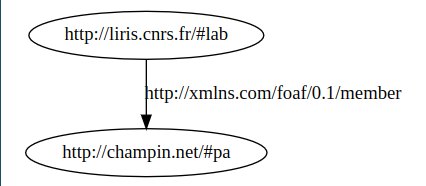
\includegraphics[width=\textwidth] {medias/schema_rdf.png}}
	\caption{Exemple de triplet en RDF}
\end{figure}

Ces innovations ont permis de poser les bases d’une interopérabilité sémantique, où des systèmes différents peuvent échanger et comprendre des données dans un langage commun.\newline

Malgré les avancées théoriques, la mise en pratique de ces concepts a rencontré plusieurs défis. D’une part, le coût élevé des technologies associées au web sémantique a freiné l’adoption de ces outils, en particulier dans les institutions culturelles disposant de ressources limitées. D’autre part, les compétences techniques nécessaires pour implémenter ces solutions ont également constitué un obstacle majeur. Les musées, en particulier, ont dû relever un défi supplémentaire : celui de l’adaptation des standards globaux aux réalités locales de leurs collections et de leurs pratiques. \newline

Ainsi, la science de l’information a progressivement évolué pour répondre à ces nouveaux défis numériques, mais elle a également montré ses limites. Le besoin de solutions pragmatiques et adaptées aux contextes variés des institutions culturelles a conduit à l’émergence de modèles spécifiques, comme LIDO ou CIDOC CRM, qui seront explorés plus en détail dans les parties suivantes. Ces modèles visent à combler l’écart entre la théorie et la pratique, en offrant des solutions de normalisation qui prennent en compte la diversité des collections et des pratiques des musées.\newline

\textbf{Les promesses et les limites des technologies du web sémantique dans les institutions culturelles}\newline

Le web sémantique a apporté de nombreuses promesses aux institutions culturelles, notamment en facilitant l’interconnexion des données à travers des systèmes disparates. En théorie, cette technologie permet de surmonter les barrières qui séparaient autrefois les différentes institutions et leurs bases de données, en créant un réseau sémantique où chaque objet numérique est relié à d’autres informations, qu’elles soient locales ou externes à l’institution.\newline

L’une des principales forces du web sémantique réside dans sa capacité à connecter les données en utilisant des formats normalisés et des ontologies communes. Par exemple, une œuvre d’art numérisée dans un musée peut être liée à des informations biographiques sur l’artiste, disponibles dans une autre base de données. Ce type de connexion transversale permet non seulement de donner plus de contexte à chaque objet, mais aussi de faciliter des recherches plus complexes, où les utilisateurs peuvent naviguer d’une œuvre à une autre en suivant des liens sémantiques.\newline

Un autre avantage clé du web sémantique est la possibilité d'automatiser certaines tâches de recherche et d'organisation des données. Grâce à des technologies comme le SPARQL, il est possible d'interroger des bases de données en réseau et d’obtenir des résultats qui combinent des informations provenant de différentes sources. Cela ouvre la voie à des recherches plus puissantes et à des découvertes qui auraient été impossibles dans un cadre plus cloisonné. Pour les musées, cela signifie une opportunité de mieux valoriser leurs collections, en les rendant plus accessibles et plus interconnectées avec d'autres institutions. \newline

Toutefois, malgré ces avantages théoriques, l’adoption du web sémantique dans les institutions culturelles a été ralentie par plusieurs facteurs. Tout d’abord, la complexité technique des technologies associées au web sémantique a constitué un obstacle majeur. Pour implémenter des systèmes basés sur des ontologies et des modèles sémantiques, les musées doivent disposer de compétences techniques spécifiques, souvent coûteuses. De nombreuses institutions, en particulier les plus petites, n’ont ni les ressources humaines ni les moyens financiers pour adopter ces technologies à grande échelle.\newline

De plus, la diversité des collections et des pratiques entre les institutions culturelles pose un défi supplémentaire. Chaque musée possède ses propres particularités, ses propres systèmes de gestion, et souvent des méthodes d’indexation et de description qui varient considérablement d’un établissement à l’autre. Cette diversité rend difficile l’adoption d’un modèle universel qui conviendrait à toutes les institutions. Même avec des modèles normalisés comme LIDO ou CIDOC CRM, chaque musée doit adapter le modèle à ses propres besoins, ce qui complique l’interopérabilité.
Enfin, l'une des limites inhérentes du web sémantique est qu'il repose sur la qualité des données qui sont intégrées dans le système. Si les données sont mal structurées, incomplètes ou obsolètes, même les meilleures technologies ne peuvent produire des résultats satisfaisants. La qualité des métadonnées devient donc un enjeu crucial pour garantir le succès des projets de web sémantique dans les musées.\newline

Le décalage entre les promesses initiales du web sémantique et la réalité de son adoption dans les musées nous conduit à une réflexion plus large sur la manière dont ces technologies peuvent être adaptées aux besoins des institutions culturelles. Il est clair que si le web sémantique offre des possibilités immenses, il doit être accompagné de processus de normalisation rigoureux, mais aussi de solutions adaptées aux réalités pratiques et économiques des musées. Cela nécessite une coopération étroite entre les développeurs de technologies, les experts en gestion de collections, et les décideurs culturels.


\chapter{L’histoire de la normalisation des données dans les musées.}
\subsection{Historique de la normalisation dans les musées français.}
Comparés aux bibliothèques et aux archives, les musées ont adopté les pratiques de normalisation avec un certain retard. Cependant, un certain nombre d’institutions semblent avoir pris conscience de cet enjeu, notamment avec la multiplication des initiatives de numérisation des collections.\footcite{numerisation} En France, le Service des Musées de France (SMF) a joué un rôle capital dans la promotion de la numérisation des collection et de la normalisation des données muséales. Fondé en 2009 pour succéder à la Direction des musées de France, il a imposé des normes pour l’inventaire et le récolement des collections. \footcite{art_4_2020} \footcite{loi_2002} Ce processus a permis d’intégrer les collections des musées de France dans des catalogues collectifs, facilitant ainsi leur gestion et leur valorisation à l’échelle nationale.\newline

\textbf{Le récolement : un enjeu de normalisation et de gestion des collections}\newline

Le récolement, c’est-à-dire la vérification périodique des collections, est une procédure imposée par la loi pour les musées de France. Cette procédure est un exemple concret de la normalisation appliquée à la gestion des collections. Elle permet non seulement de vérifier l’état et l’existence des objets, mais aussi de mettre à jour les informations les concernant, assurant ainsi la qualité et l’exactitude des données dans les systèmes d’information des musées. Il permet aussi parfois de se rendre compte d’anomalies, comme des détériorations d’un objet, une disparition, ou un manque d’information (pas d’acte d’entrée dans les collections par exemple).\newline

Le récolement implique de « vérifier, sur pièce et sur place, à partir d'un bien ou de son numéro d'inventaire, la présence du bien dans les collections, sa localisation, son état, son marquage, la conformité de l'inscription à l'inventaire avec le bien et, le cas échéant, avec les différentes sources documentaires, archives, dossiers d'œuvre, catalogues ». (Décret du 25 mai 2004 établissant les règles techniques concernant la gestion de l'inventaire, le registre des biens déposés dans un musée de France et le récolement).\newline

Le récolement suit des normes techniques fixées par l’Arrêté du 25 mai 2004. Ainsi, pour chaque objet récolté, on doit disposer au minimum de certaines données, comme la date d’acquisition, le numéro d’inventaire, etc…\newline

Le récolement est devenu obligatoire et systématique depuis la loi de 2002 sur les musées de France. Cette dernière a imposé de faire le récolement complet des collections tous les dix ans (on parle de récolement décennal). Il s’agit d’une mission permanente.\footcite{recolement}\newline

L'évolution de la documentation des collections muséales.\newline

\begin{quote}
    <<C’est avec la mise en place de bases de données dédiées à l’administration et à la gestion de la collection que les technologies informatiques et les politiques de numérisation entrent au musée. Traditionnellement reportés dans un cahier d’inventaire, les artefacts d’une collection sont reliés à tout élément documentaire et de gestion par un numéro, le numéro d’inventaire. La base de données informatique fonctionnant sur un principe identique (un numéro reliant des fiches contenant elles-mêmes des champs associés à un même sujet), elle devient l’outil idéal de gestion des collections. Ce premier pas désigné comme l’informatisation ou la numérisation des collections aura des conséquences sur la production des contenus associés aux artefacts ainsi que sur leur mise en forme. La base de données informatisée va permettre d’entrer dans la collection par de nouvelles entrées. À la requête par numéro d’inventaire, s’ajoutera l’emploi de thésaurus et autres systèmes de descripteurs.>> \footcite{andreacola_2014}
\end{quote}
L’histoire de la normalisation dans les musées remonte à plusieurs siècles, bien avant l’avènement du numérique. Dans les premières phases de développement des musées, la documentation des collections se faisait de manière très locale. Chaque institution avait son propre système de catalogage, qui consistait souvent en des registres, manuels ou des livres d’inventaire. Ces documents, bien que précieux, avaient des limites évidentes : ils étaient statiques, difficiles à mettre à jour, et surtout peu compatibles d’une institution à l’autre. Si un chercheur voulait consulter les informations sur une collection dans un autre musée, il devait se déplacer physiquement et se plonger dans les registres souvent non standardisés.\newline

Cette situation a perduré jusqu’à l’émergence des normes internationales en matière de gestion de l’information culturelle. Les bibliothèques et les archives ont été les premières à développer des standards pour la description des documents, avec des initiatives comme MARC pour les bibliothèques dans les années 1960. Les musées, quant à eux, ont pris du retard dans l’adoption de pratiques similaires, en raison de la complexité et de la diversité des objets qu’ils gèrent. Contrairement aux livres ou aux documents d’archives, qui sont souvent structurés de manière similaire, les objets de musée peuvent être extrêmement variés, allant des œuvres d’art aux artefacts historiques, en passant par les objets ethnographiques, scientifiques ou industriels.\newline

Cette diversité a compliqué la tâche de normalisation, car chaque type d’objet nécessite des méthodes de description spécifiques. Par exemple, décrire un tableau implique de mentionner des informations sur l’artiste, le matériau utilisé, et l’école artistique, tandis qu’un artefact archéologique peut nécessiter des informations sur son contexte de découverte, son lieu d’origine, et son utilisation historique. Cette hétérogénéité a retardé l’adoption de normes communes, chaque musée développant souvent son propre système de gestion des collections.\newline

L'impact de la normalisation internationale : le CIDOC CRM et LIDO
L’un des tournants majeurs dans l’histoire de la normalisation des données muséales a été la création du CIDOC CRM (Conceptual Reference Model) dans les années 1990 par le Conseil International des Musées (ICOM). Ce modèle conceptuel a été conçu pour répondre aux besoins des musées en matière de documentation des collections. Contrairement à des modèles plus simples comme MARC, le CIDOC CRM prend en compte la complexité des objets muséaux et des événements associés à ces objets (leur création, leur usage, leur acquisition, etc.).\newline

Le CIDOC CRM offre un cadre flexible qui permet de modéliser non seulement les objets eux-mêmes, mais aussi leur contexte historique et les événements auxquels ils sont liés. Par exemple, il peut décrire un tableau non seulement comme un objet physique, mais aussi en tant que témoin d’un événement artistique (l’acte de peindre), tout en prenant en compte les relations entre l’artiste, le commanditaire, le lieu de création, et l’œuvre elle-même. Ce modèle permet donc de capturer la richesse des collections muséales, en tenant compte des différentes couches d’information qui entourent chaque objet. \newline

Cependant, le CIDOC CRM, bien qu’efficace, est aussi un modèle complexe qui demande des compétences techniques pour être mis en œuvre et même pour être compris par les responsables de gestion interne aux musées. De nombreux musées, en particulier les plus petits, n’ont pas les ressources nécessaires pour adopter ce modèle dans sa totalité. C’est pourquoi des alternatives plus simples ont été développées pour faciliter l’adoption de normes sans pour autant sacrifier la richesse des données. Mais il faut souligner qu’en France les musées ne s’appuient pas forcément sur des modèles de données communs, mais plutôt sur les possibilités proposées par les logiciels de gestion des collections. \newline

C’est dans ce contexte qu’est né le modèle LIDO (Lightweight Information Describing Objects). Développé également par l’ICOM, LIDO est conçu pour être un modèle léger et facile à utiliser, tout en conservant la capacité de décrire des objets complexes. Contrairement au CIDOC CRM, qui est un modèle conceptuel, LIDO est un schéma XML directement exploitable dans les systèmes de gestion de collections. Il est adapté à au transport de données, à leur collecte et donc l’agrégation des données, c’est-à-dire à la collecte de données provenant de différentes sources pour les diffuser à travers des plateformes partagées, comme Europeana ou la plateforme française POP.\newline

LIDO permet aux musées de standardiser la description de leurs collections de manière simple et efficace. Par exemple, un musée peut utiliser LIDO pour exporter ses données vers une plateforme nationale ou internationale, garantissant ainsi que les informations partagées sont conformes aux demandes de celles-ci. Le LIDO peut aussi être utilisé pour faire le lien entre différentes institutions entre elles, lors de prêts pour des expositions par exemple. LIDO prend en charge des éléments essentiels de la description d’objets, tels que le titre, l’artiste, la date de création, le matériau, les dimensions, ainsi que des informations sur les droits et l’accès aux œuvres. En ce sens, LIDO est un outil puissant pour répondre aux besoins d’interopérabilité, tout en étant plus accessible que des modèles plus complexes comme le CIDOC CRM. \newline

\textbf{Les défis de l’adoption des standards de données culturelles en France.}\newline

En France, la normalisation des données muséales a été portée par des initiatives gouvernementales, notamment sous l’impulsion du Ministère de la Culture. Le Service des Musées de France (SMF) a joué un rôle clé dans la promotion de la standardisation à l’échelle nationale. Le SMF est responsable de l’encadrement de la gestion des musées de France, un réseau qui regroupe environ 1 200 musées sur l’ensemble du territoire français.\newline

L’un des premiers efforts de normalisation en France a été la création de la base de données Joconde, qui regroupe les collections des musées français sous un format standardisé. Joconde a été conçue comme une plateforme nationale permettant de centraliser les informations sur les collections des musées, de les rendre accessibles au grand public et aux chercheurs, et de faciliter la collaboration entre les institutions. Cette initiative a marqué un tournant dans la manière dont les musées français gèrent leurs collections, en introduisant un format d’export standardisé pour la description des objets. \newline

Aujourd’hui pour être intégrée à la base Joconde et diffusée sur POP, une notice d’objet doit respecter une certaine forme. Cette forme implique une rigueur scientifique puisque la notice doit comporter un minimum d’information. Parmis ces données obligatoires on compte le numéro d’inventaire, le domaine (vocabulaire contrôlé), et le statut juridique. D’autres données ne sont pas signalées comme obligatoires mais comme indispensables, c’est le cas pour la désignation, les mesures ou le lieu de conservation, entre autres.\newline

Cependant, malgré ces avancées, la diversité des pratiques reste un défi majeur pour l’adoption des standards en France. Chaque musée, qu’il soit national, régional ou local, a ses propres méthodes de gestion des collections, souvent en fonction des ressources disponibles et de la nature de ses collections. Certains musées, notamment les plus petits, n’ont pas toujours les moyens de mettre en place des systèmes de gestion sophistiqués, et continuent d’utiliser des méthodes plus traditionnelles ou des solutions informatiques non standardisées.\newline

De plus, la diversité des fournisseurs de logiciels pour la gestion des collections complique l’adoption de standards communs. De nombreux musées utilisent des logiciels propriétaires développés par des entreprises spécialisées, qui ne sont pas toujours compatibles avec les normes nationales ou internationales. Cette situation conduit à une diversité de mode de description des œuvres et donc à fragmentation des données, chaque musée ayant son propre système de gestion, ses propres structurations de leur base de données des collections et de leur mode de description, et ses propres pratiques de documentation. Cela rend difficile l’intégration de ces données dans des plateformes partagées comme POP, qui exige des formats standardisés. Qui plus est, l'obligation de récolement décennal rend le processus de partage de données vers POP, très lourd administrativement et le versement des données est souvent ralenti car les données ne sont pas à jour si récolement pas terminé. Des échanges avec des professionels nous on permis d'estimer que pour certaines institutions muséales le retard potentiel serait de 10 ans ou plus sur les informations disponible sur le portail.\newline

Pour répondre à ces défis, le Ministère de la Culture a mis en place des recommandations pour encourager les musées à adopter des standards communs, en particulier LIDO. Des formations sont également proposées pour aider les musées à s’adapter aux nouvelles exigences de l’interopérabilité et de la gestion des données numériques. L’objectif est de créer un écosystème unifié, où toutes les institutions peuvent partager leurs données de manière fluide et efficace, tout en préservant la spécificité de leurs collections.

\subsection{Les formes de normalisation des données muséales en France et à l’étranger
L’export Joconde : un format d'export spécifique aux musées français}

\textbf{L’agrégation des données culturelles et la plateforme POP}\newline

POP est une initiative du Ministère de la Culture qui vise à centraliser les données sur le patrimoine culturel français, en regroupant les informations provenant de différentes bases de données comme Joconde pour les musées. Celle-ci existe depuis 1975 et ses données ont été mises en ligne dans les années 90. POP aussi accès aux bases Palissy pour le patrimoine mobilier, Mérimé pour le patrimoine architectural, Enluminure pour les enluminures, et d’autres. \footcite{base_Joconde}

POP permet de diffuser les données culturelles à l’échelle nationale, en offrant un point d’accès unique aux collections des musées, aux monuments historiques, et aux archives patrimoniales. Les musées peuvent ainsi publier leurs collections sur POP, en garantissant que les informations sont accessibles au grand public, aux chercheurs, et aux autres institutions culturelles.
Ce portail permet de rendre visible des collections qui, autrement, resteraient confinées dans les bases de données internes des musées. Les petites institutions, qui n’ont pas toujours les moyens de diffuser leurs collections sur des plateformes propres, peuvent bénéficier de la visibilité offerte par POP. De plus, en centralisant les données, POP facilite les recherches transversales entre différentes collections, permettant aux utilisateurs de découvrir des liens entre des objets provenant de différents musées ou régions.
Cependant, le succès de POP dépend de la qualité des données qui y sont agrégées. Pour que la plateforme soit pleinement efficace, il est crucial que les données soient bien structurées, complètes, et conformes aux standards. C’est pourquoi la normalisation des données reste un enjeu fondamental pour le bon fonctionnement de cette plateforme et pour garantir la pérennité des informations qu’elle contient.
		

\textbf{L’export Joconde}: un format d'export de données spécifique aux musées français
En France, l’export Joconde représente une forme spécifique de normalisation des données muséales. Ce format est utilisé pour l’intégration des collections dans la base Joconde, le catalogue collectif des musées de France. Cependant, cette normalisation n’est pas appliquée de manière homogène à travers tous les musées, ce qui pose des défis en termes d’interopérabilité et de partage des données. Certains musées ont développé des solutions propres, ce qui complique la création d’un cadre normatif commun.\newline

L'export Joconde est en fait de le format d'export qui sort de la base Joconde. Mais pour pouvoir l'intégrer et vois ses données diffusées sur POP, les musées doivent s'y conformer.\newline

Il s'agit en fait d'une liste champs spécifique dont certains ont l'obligation d'être renseignés. Les données doivent être structurées selon ces champs. \footcite{muséofile} \footcite{base_Joconde} \footcite{Joconde}

\begin{longtable}{|p{7cm}|p{5cm}|}
\hline
\textbf{Intitulé de champ Joconde} & \textbf{Étiquette de champ Joconde} \\
\hline
Référence & REF \\
POP\_CONTIENT\_GEOLOCALISATION & disponible ou non
\\
POP\_COORDONNEES & base Muséofile\\
Ancien dépôt & ADPT \\
Appellation & APPL \\
Ancienne appartenance & APTN \\
Ancienne attribution & ATTR \\
Auteur & AUTR \\
Base concernée & BASE \\
Bibliographie & BIBL \\
Commentaires & COMM \\
Présence d’image (s) oui/non & CONTIENT\_IMAGE \\
Copyright de la notice & COPY \\
Date d’acquisition & DACQ \\
Date de dépôt & DDPT \\
Découverte-collecte & DECV \\
Dénomination & DENO \\
Lieu de dépôt & DEPO \\
Description & DESC \\
Mesures & DIMS \\
Date de mise à jour & DMAJ \\
Date de création & DMIS \\
Domaine & DOMN \\
Département & DPT \\
Date sujet représenté & DREP \\
Ecole-pays & ECOL \\
Époque & EPOQ \\
État du bien & ETAT \\
Exposition & EXPO \\
Genèse & GENE \\
Géographie historique & GEOHI \\
Historique & HIST \\
HISTORIQUE & Historique des interventions manuelle ou export de données
\\
IMAGE & oui ou non\\
Inscription & INSC \\
Numéro d’inventaire & INV \\
Appellation musée de France & LABEL \\
Lien base Arcade & LARC \\
Lieux de création / utilisation & LIEUX \\
Localisation & LOCA \\
Pays Région Ville & LOCA2 \\
Lien Vidéo & LVID \\
Bien manquant & MANQUANT \\
Commentaire & MANQUANT\_COM \\
Millésime de création & MILL \\
Millésime d’utilisation & MILU \\
Lien commande photo & MSGCOM \\
Code Museofile & MUSEO \\
Nom officiel du musée & NOMOFF \\
Onomastique & ONOM \\
Précisions auteur & PAUT \\
Précisions découverte/collecte & PDEC \\
Période de l’original copié & PEOC \\
Période de création & PERI \\
Période d’utilisation & PERU \\
Crédits photographiques & PHOT \\
Précisions inscriptions & PINS \\
Précisions lieux de création & PLIEUX \\
Précisions sujet représenté & PREP \\
Producteur de la donnée & PRODUCTEUR \\
Précisions utilisation & PUTI \\
Références Mémoire liées & REFMEM \\
Références Mérimée liées & REFMER \\
Référence MAJ & REFMIS \\
Références Palissy liées & REFPAL \\
Sujet représenté & REPR \\
Lien INHA & RETIF \\
Source représentation & SREP \\
Statut juridique & STAT \\
Matériaux-techniques & TECH \\
Titre & TITR \\
Utilisation & UTIL \\
Ville & VILLE\_M \\
Lien site associé & WWW \\
\hline
\end{longtable}

\textbf{Les initiatives internationales} : un modèle à suivre ?\newline

Dans les pays anglo-saxons, des standards comme le Dublin Core et le CIDOC CRM (Conceptual Reference Model) ont été largement adoptés pour la gestion des collections muséales. Le Dublin Core est un schéma de métadonnées utilisé pour décrire diverses ressources numériques, y compris les objets de musée. Il offre une flexibilité tout en assurant une structure commune, ce qui facilite l'échange d'informations entre institutions. \newline

Le CIDOC CRM, quant à lui, est un modèle conceptuel qui permet de structurer et d’interconnecter des informations complexes sur le patrimoine culturel. Par exemple, ce modèle permet de relier des informations sur un même objet réparties entre plusieurs bases de données, facilitant ainsi les recherches et les études comparatives. Il s'agit d'une initiative inernationale qui devait permettre de pouvoir faire des liens entre des données du monde entier, mais comme nous l'avons évoqué plus tôt, son usage est loin d'être démocratisé.\newline

\textbf{Vers une harmonisation internationale des pratiques ?}\newline
L'adoption de ces standards à l’échelle internationale montre une tendance vers une harmonisation des pratiques de normalisation. Toutefois, des disparités persistent, en partie à cause des spécificités culturelles et institutionnelles de chaque pays. Par exemple, la France, avec son système d'export Joconde, illustre bien comment des pratiques nationales peuvent coexister avec des standards internationaux, tout en cherchant à les harmoniser progressivement. \newline

La normalisation des données est un processus fondamental qui a évolué au fil du temps, des répertoires papier aux technologies numériques avancées. Dans le domaine des collections culturelles, cette normalisation a permis de structurer, d’organiser et de rendre accessible un vaste ensemble d’informations. Alors que les musées ont adopté ces pratiques plus tardivement que d’autres institutions culturelles comme les bibliothèques, ils jouent désormais un rôle central dans le développement de standards internationaux, avec des initiatives comme le LIDO ou le CIDOC CRM.\newline

Les défis restent nombreux, notamment en ce qui concerne l'interopérabilité entre les différentes plateformes et la diversité des pratiques nationales. Toutefois, les progrès réalisés montrent une tendance vers une plus grande cohésion, facilitée par les avancées technologiques et les efforts concertés des institutions culturelles à travers le monde.


%Input: importer un fichier
%\input{ma_section2}

%etc
%Ou bien: ne pas mettre chapter, et importer le chapitre complet:
%\input{mon_chapitre_1.tex}
%\input{mon_chapitre_2.tex}	
%etc
	
	\part{Les Standards dans métiers, quels -sont-ils et pour quoi sont-t’ils utilisées, objectifs de l’agrégation.}
 \chapter{Les Modèles de Données : MARC, EAD, et le Lien avec la diffusion.}
 \subsection{Introduction aux Modèles de Données : MARC et EAD}

Les modèles de données sont des schémas standardisés utilisés pour structurer et organiser les informations dans le domaine du patrimoine culturel. Parmi les plus courants, on trouve le format MARC (Machine-Readable Cataloging) et le format EAD (Encoded Archival Description). \newline

Le format MARC, créé dans les années 1960, est un modèle de données utilisé principalement dans les bibliothèques pour la description des ressources bibliographiques. Ce format permet de structurer les informations de manière à ce qu'elles soient lisibles par des machines, facilitant ainsi l'échange de données entre institutions. En revanche, le format EAD, apparu dans les années 1990, est destiné aux archives. Il permet de structurer la description des collections archivistiques de manière hiérarchique, rendant ainsi possible la recherche et la navigation au sein de ces collections.\newline

L’un des premiers modèles adoptés dans les bibliothèques et les archives est le MARC (Machine-Readable Cataloging), un format de description normalisé qui a été développé dans les années 1960 par la Bibliothèque du Congrès aux États-Unis. Ce modèle permet de décrire de manière uniforme les documents bibliographiques et a été largement adopté par les bibliothèques à travers le monde. Il a constitué la base pour le développement d’autres modèles plus récents, comme le Dublin Core, qui a été conçu pour être un modèle plus léger et plus adapté aux besoins du web sémantique.
Le Dublin Core est un schéma de métadonnées simple qui permet de décrire les objets numériques à travers 15 éléments de base, comme le titre, l’auteur, la date de création, le sujet, et la description. Ce modèle a été adopté dans de nombreux contextes, notamment pour la description des objets culturels dans des environnements numériques. Cependant, il reste limité en termes de granularité et de capacité à décrire des objets complexes, ce qui a conduit à la création de modèles plus spécialisés pour les musées, comme CIDOC CRM et LIDO.\newline

Ces modèles de données sont essentiels car ils permettent de passer de la donnée brute, souvent complexe et difficile à exploiter, à une information structurée et normalisée. Ce processus est crucial pour la diffusion et l’accessibilité des données sur le web, où l'interopérabilité des systèmes est une exigence fondamentale. \newline

\textbf{Le Lien entre Donnée Brute et Diffusion : L'Importance des Modèles Structurés}
Dans un contexte numérique, la donnée brute doit être transformée pour être exploitable dans des systèmes de diffusion. Cette transformation repose sur l’application de modèles de données comme MARC et EAD. Par exemple, une notice bibliographique en MARC peut être facilement partagée entre bibliothèques, tandis qu'une description archivistique en EAD peut être intégrée dans un portail d'archives en ligne. Cette interopérabilité est rendue possible grâce à la normalisation des données.\newline

En effet, un modèle de données permet de définir les champs et les valeurs possibles pour chaque type d'information, assurant ainsi que chaque donnée est conforme à un standard commun. Cela facilite non seulement la diffusion, mais aussi la recherche et la réutilisation des données à travers différentes plateformes. Les utilisateurs peuvent ainsi accéder à des informations provenant de multiples institutions, sans se soucier des différences de format ou de structure. \newline

Exemples Concrets d'Utilisation : MARC, EAD et leur Impact
L'utilisation de MARC dans les bibliothèques et d'EAD dans les archives a permis une révolution dans la manière dont les informations sont partagées et diffusées. Par exemple, la Bibliothèque nationale de France (BnF) utilise le format MARC pour cataloguer et diffuser ses collections via le portail Gallica. De même, les Archives nationales de France utilisent le format EAD pour structurer et publier leurs inventaires en ligne, rendant ainsi les documents archivistiques plus accessibles au public et aux chercheurs.\newline
Les modèles de données comme MARC et EAD sont des outils indispensables pour structurer et diffuser les informations culturelles sur le web. Ils permettent de transformer des données brutes en informations structurées, facilitant ainsi leur partage, leur recherche et leur réutilisation.\newline

Ces deux modèles que nous avont présenté, sont majoritairement utilisés par les bibliothèques et les services d'archives, nous allons maintenant nous intérresser aux musées.


 \subsection{Les Modèles de Données dans les Musées : Un État des Lieux}
\textbf{Contexte Actuel des Modèles de Données dans les Musées}\newline

Dans le domaine muséal, la question de la normalisation et de la structuration des données est devenue cruciale à mesure que les institutions cherchent à améliorer la gestion et la diffusion de leurs collections. Plusieurs modèles de données ont été développés pour répondre à ces besoins, chacun avec ses spécificités et ses objectifs. Parmi les plus notables utilisés en France, on trouve le Dublin Core, l'export Joconde, le CIDOC CRM et diverses ontologies spécifiques.\newline

Le Dublin Core est un schéma de métadonnées simple, il peut être utilisé dans le milieu muséal pour décrire les objets culturels. Il est particulièrement apprécié pour sa simplicité et sa flexibilité, ce qui permet une adoption facile par les institutions, même celles qui disposent de ressources limitées.\newline


\begin{longtable}{|p{4cm}|p{4cm}|p{8cm}|}
\hline
\textbf{Élément} & \textbf{Élément (anglais)} & \textbf{Commentaire} \\
\hline
1. Titre (métadonnée) & Title & Nom donné à la ressource \\
\hline
2. Créateur (métadonnée) & Creator & Nom de la personne, de l'organisation ou du service responsable de la création du contenu de la ressource \\
\hline
3. Sujet (métadonnée) ou mots clés & Subject & Thème du contenu de la ressource (mots clés, expressions, codes de classification) \\
\hline
4. Description (métadonnée) & Description & Présentation du contenu de la ressource (résumé, table des matières, représentation graphique du contenu, texte libre) \\
\hline
5. Éditeur & Publisher & Nom de la personne, de l'organisation ou du service responsable de la mise à disposition ou de la diffusion de la ressource \\
\hline
6. Contributeur & Contributor & Nom de la personne, de l'organisation ou du service responsable de contributions au contenu de la ressource \\
\hline
7. Date (métadonnée) & Date & Date de création ou de mise à disposition de la ressource \\
\hline
8. Type & Type & Nature ou genre de la ressource (catégories, fonctions, genres généraux, niveaux d'agrégation du contenu) \\
\hline
9. Format & Format & Manifestation physique ou numérique de la ressource \\
\hline
10. Identifiant de la ressource & Identifier & Référence univoque à la ressource dans un contexte donné (URI, ISBN) \\
\hline
11. Source & Source & Référence à une ressource dont la ressource décrite est dérivée (URI) \\
\hline
12. Langue (métadonnée) & Language & Langue du contenu intellectuel de la ressource \\
\hline
13. Relation (métadonnée) & Relation & Référence à une ressource apparentée \\
\hline
14. Couverture (métadonnée) & Coverage & Couverture spatio-temporelle de la ressource (domaine d'application) \\
\hline
15. Gestion de droits (métadonnée) & Rights & Informations sur les droits associés à la ressource (IPR, copyright, etc.) \\
\hline
\end{longtable}


L'export Joconde, quant à lui, est un format spécifiquement développé pour les musées français. Il permet de structurer les informations relatives aux objets des collections de manière à ce qu'elles puissent être intégrées dans la base Joconde, le catalogue collectif des musées de France. Ce format est essentiel pour la mutualisation des données à l'échelle nationale, assurant ainsi une visibilité accrue des collections et une diffusion accrue et efficace.\newline

Le CIDOC CRM (Conceptual Reference Model) que nous avons déjà présenté est un modèle conceptuel élaboré par le Comité international pour la documentation (CIDOC) du Conseil international des musées (ICOM). Il vise à modéliser les relations complexes entre les objets, les événements et les personnes dans le domaine du patrimoine culturel.\newline

Enfin, les ontologies spécifiques aux musées, comme celles développées pour les objets ethnographiques ou les œuvres d'art, permettent de structurer les données en fonction des particularités de chaque type de collection. Ces ontologies facilitent l'intégration des données dans des systèmes de gestion complexes, tout en assurant une cohérence et une précision accrues.\newline

\textbf{Exemples Pratiques et Impact sur la Qualité des Données}\newline

Au cours de notre stage nous avons rencontré différents cas d’usages. En effet, dans le cadre de notre mission au sein du DPNC (sous direction du Service du numérique, Département du numérique pour la transformation des politiques culturelles et de l'administration des données)nous avons participé à l’animation du réseau des agrégateurs intermédiaires. Ces entités agrègent les données de plusieurs institutions culturelles et les diffusent sur des portails et des sites internets. Ces agrégateurs réunissent les données d'institutions selon des critères qui peuvent être thématiques ou géographiques. \newline

Nous avons notamment pu échanger avec des représentants du portail Bretania, qui agrège et diffuse des données d'institutions culturelles en Bretagne telles que  la Cinémathèque de Bretagne, les différents musées et les archives municipales, entre autres. La Base Aliénor et la DRAC PACA, réunissent eux aussi des données relevant du patrimoine culturel à l’échelle de leur région. Nous avons également échangé avec des représentants du projet de portail thématique Graph Ethno, un portail des collections des écomusées et musées de société en France qui à pour objectif de créer un réseau de valorisation numérique des collections de ces institutions. \newline

Dans le projet d’agrégation du ministère, le but n’est pas de se limiter aux institutions muséales, c’est pour cette raison que nous avons également pu échanger avec des représentants de la Réunion des Opéras de France et de la Philharmonie de Paris. 
Chacun des agrégateurs que nous avons pu rencontrer à des pratiques différentes pour agréger et gérer ses données. Voici quelques exemples auxquels nous avons fait face. \newline

Le cas de la Réunion des Opéras de France (ROF) et CapData Opéra : 
La ROF mène depuis 2O22 le projet CapData Opéra, c’est un projet qui utilise les technologies du Web sémantique comme fondement d’une solution de structuration et de diffusion des données culturelles capable de répondre aux besoins des institutions. Cette initiative est portée par la ROF avec le soutien du Ministère de la Culture et de plusieurs partenaires techniques, tels que Logilab (une société qui développe des logiciels, de préférence libres, et propose du conseil et des formations dans les domaines du web sémantique et de l'informatique scientifique). Cette solution de mutualisation permet d’interroger les données produites par plusieurs acteurs du domaine pour, par exemple, connaître la programmation et la circulation d’une œuvre ou d’une production entre plusieurs maisons d’opéra. Ce projet réunit les donnés de six maisons d’opéra et s’appuie sur les technologies du Web sémantique et notamment sur le standard RDF (Resource Description Framework). Ce projet a aboutit à la publication de l‘ontologie CapData Opéra. \newline
L'objectif est de centraliser et de standardiser les informations, facilitant ainsi leur partage et leur utilisation par des publics variés, incluant les opéras, les développeurs, et les acteurs culturels.\newline

Les maisons d'opéra gèrent quotidiennement des données multiples, notamment sur leur programmation, les artistes, et les productions. Cependant, ces données sont souvent stockées dans des systèmes distincts et non interopérables, rendant difficile leur croisement et leur réutilisation à grande échelle. L'absence de standards communs pour identifier les œuvres, les artistes, ou les productions de spectacles vivants constitue un frein majeur à leur diffusion. À titre d'exemple, il n'existe pas d'équivalent à l'ISBN (livres) ou à l'ISRC (industrie musicale) pour identifier les productions de spectacle vivant, compliquant la tâche des maisons d’opéra souhaitant partager leurs données avec d’autres plateformes. \newline

Le projet CapData Opéra se donne pour mission de résoudre ces problèmes d'interopérabilité en créant une infrastructure mutualisée qui permet aux maisons d’opéra de publier et de partager leurs données de manière standardisée. Cette infrastructure repose sur les technologies du Web Sémantique et notamment sur le standard RDF (Resource Description Framework), un format conçu pour représenter les données de manière structurée et facilitant leur interconnexion.
Le projet vise à répondre à plusieurs enjeux clés :
Interopérabilité accrue des données : permettre aux maisons d'opéra de partager facilement leurs informations avec d'autres institutions et acteurs culturels.
Réduction des saisies manuelles : minimiser les doublons et les erreurs de saisie en automatisant la structuration et la diffusion des données.
Facilitation de la découvrabilité : accroître la visibilité des œuvres, artistes, et productions auprès des publics via des plateformes numériques, des moteurs de recherche, ou des services innovants.
Souveraineté des données : permettre à chaque maison d'opéra de conserver le contrôle sur ses propres données tout en facilitant leur partage avec d'autres. \newline

Pour structurer et diffuser les données, CapData Opéra s'appuie sur une ontologie dédiée qui définit un vocabulaire commun entre les différents opéras. Cette ontologie est conçue pour s'aligner avec des modèles de données existants, notamment schema.org, utilisé pour la découvrabilité sur le web, et l’ontologie IFLA-LRM, bien adaptée aux ressources bibliographiques. Cependant, certaines lacunes ont été identifiées dans ces modèles, notamment en ce qui concerne la description fine des productions artistiques, ce qui a conduit au développement d’une ontologie propre à CapData Opéra.
Une partie clé du projet repose sur le développement d’un outil appelé Rodolf, conçu pour suivre la publication et la structuration des données RDF. Rodolf permet aux maisons d'opéra de suivre les fichiers de données publiés, d'identifier d'éventuelles erreurs, et de vérifier la validité des données à travers un ensemble de règles SHACL (Shapes Constraint Language). En outre, un kit de développement logiciel (SDK) a été mis à disposition pour faciliter l’export des données en RDF, même pour les développeurs peu familiers avec les technologies du Web Sémantique. \newline

Depuis son lancement en 2022, CapData Opéra a d'abord été testé avec l'Opéra National de Bordeaux et d'autres partenaires. Les premiers résultats montrent une nette amélioration de la capacité à croiser les données entre les opéras et à diffuser les informations de manière cohérente et automatisée. Le projet a également permis de créer des liens avec des initiatives internationales similaires, notamment dans le domaine des arts vivants et du spectacle.
En plus de faciliter la publication et la circulation des données, cette approche a aussi permis d'améliorer la qualité des informations stockées par chaque maison d'opéra. Grâce aux outils développés, les opéras peuvent désormais enrichir leurs propres bases de données avec des informations normalisées, telles que les identifiants ISNI (International Standard Name Identifier) pour les artistes. \newline

Le projet CapData Opéra représente une avancée significative pour la gestion des données dans le secteur des arts vivants, et notamment pour les maisons d'opéra. En s’appuyant sur les technologies du Web Sémantique et une ontologie dédiée, il facilite la standardisation et la diffusion des données tout en respectant la souveraineté de chaque institution. À terme, cette initiative pourrait s’étendre à d’autres types d’institutions culturelles, comme les théâtres, et contribuer à une meilleure visibilité des créations artistiques à travers les plateformes numériques et les nouveaux modes de diffusion.

Le projet est encore en phase d’expérimentation et de développement, mais les résultats obtenus jusqu'à présent sont prometteurs, avec des perspectives de déploiement à grande echelle. \footcite{CapData_Opera}

\begin{figure}[h!]
	\centerline{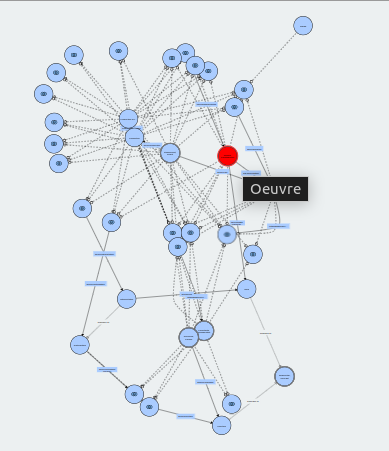
\includegraphics[width=\textwidth]{medias/capData_opera.png}}
	\caption{Apperçu du graphe de données de l'ontologie Capdata Opéra}
\end{figure}

La création d'ontologies spécifiques est également envisagée dans d'autres domaines tels que les collections d'ethnographie avec le projet GraphEthno, bien que ce dernier soit toujours en cours de développement.  Ce processus serait une solution cohérente avec la complexité des données générées par certaines de leurs institutions partenaires. Lors de nos premiers échanges c’est le Dublin Core qui leurs semblait le plus approprié pour porter les données collectées, c’est donc sous ce format que nous avons étudié leur cas. Le projet étant toujours en cours nous avons pu voir au cours des mois une évolution dans les réflexions et un intérêt pour le LIDO apparaître. \newline

Il est tout de même important de rappeler que tous les agrégateurs intermédiaires n’ont pas pour objectif de créer des ontologies. Bon nombre d’entre eux se basent sur des formats de données plus simples et choisis en fonction des données dont ils disposent. La Base Aliénor, par exemple, récupère les données en suivant les champs proposés par le format de l’export Joconde en y ajoutant des champs proposés par le Darwin Core. Le Darwin Core est une extension du Dublin Core, utilisée pour décrire avec plus de précision des objets de biodiversité.\newline

La plupart des agrégateurs intermédiaires que nous avons rencontrés n’utilisent pas de format de données standard. En effet pour produire leurs données ils s’appuient sur les informations dont ils disposent déjà dans leurs inventaires, catalogues et registres, ainsi que sur les possibilités proposées par l’éditeur de leur base de données. Le format de leurs données est donc souvent dicté par l’outil utilisé par l’institution. \newline

En conclusion, l'utilisation de modèles de données dans les musées est essentielle pour assurer la qualité, la cohérence et la diffusion des informations sur les collections. Chaque modèle a ses avantages et ses limites, mais leur adoption permet de répondre aux besoins spécifiques des musées tout en assurant une interopérabilité accrue à l'échelle nationale et internationale. Malgrés cette affirmation, nous sommes forcé de constater que, même si quleques projets montrent une évolution dans les pratiques, la majorité des données collectées par les agrégateurs intermédiaires ne suivent pas de standards communs. Les données muséales prennent surtout la forme qui est facilitée par l'outil de gestion de chaque institution utilise. 


 \chapter{ Les Autorités dans les Musées : Thésaurus et Autres Normes}
 \subsection{Les Thésaurus et Leur Contexte d'Utilisation
Définition et Importance des Thésaurus dans les Musées}

Les thésaurus sont des outils essentiels pour la normalisation des données dans les musées. Ils permettent de structurer et d'organiser les informations en utilisant des vocabulaires contrôlés, ce qui facilite la recherche, l'indexation et l'interopérabilité des données. Un thésaurus est généralement composé de termes hiérarchisés, liés à des relations synonymiques, antinomiques ou d'association, permettant ainsi de représenter de manière précise les concepts liés aux objets des collections.\newline

Dans le contexte muséal, les thésaurus sont utilisés pour décrire les objets, les techniques, les matériaux, les périodes historiques, et bien d'autres aspects des collections. Leur utilisation permet de garantir une homogénéité dans la description des objets, ce qui est crucial pour la recherche et l'agrégation des données à travers différentes institutions.\newline

\textbf{Situation Actuelle : Développements Internes et Normalisation Externe}
Actuellement, de nombreux musées développent leurs propres thésaurus en interne, adaptés aux spécificités de leurs collections. Cette approche présente l'avantage de répondre précisément aux besoins des institutions, mais elle pose également des défis en termes d'interopérabilité. En effet, ces thésaurus internes diffèrent presque systématiquement d'une institution à l'autre, ce qui complique grandement le partage et l'agrégation des données.\newline

Pour pallier ce problème, certaines institutions ont commencé à normaliser leurs thésaurus en les publiant en ligne et en les rendant accessibles à d'autres musées. Par exemple, l'ICOM et le Getty Research Institute ont développé des thésaurus largement utilisés et nommés respectivement  Getty Art \& Architecture Thesaurus (AAT)\footcite{aat-getty} et le Thesaurus of Geographic Names (TGN). 

Le Getty Thesaurus of Geographic Names (abrégé TGN) est un produit du J. Paul Getty Trust qui fait partie du Getty Vocabulary Program. Le TGN comprend des noms et des informations associées sur des lieux. Les lieux figurant dans le TGN comprennent des entités politiques administratives (des villes, des nations). Mais il comprends aussi des termes décrivant les caractéristiques physiques d'un lieu (des montagnes, des rivières). Les lieux actuels et historiques sont inclus (on pense à des entités qui n'existent plus, par exemple l'empire prussien, qui englobe des régions faisant partie de pays différents aujourd'hui). D'autres informations relatives à l'histoire, à la population, à la culture, à l'art et à l'architecture sont incluses.\footcite{thesaurus_getty_wiki}

Cette ressource est mise à la disposition des musées, des bibliothèques d'art, des archives, des catalogueurs de collections de ressources visuelles et des projets bibliographiques par le biais d'une licence privée. Elle est également disponible gratuitement pour le grand public sur le site Web du Vocabulaire Getty.

Les bases de données de vocabulaire du Getty (Art \& Architecture Thesaurus (AAT), Union List of Artist Names (ULAN), et TGN) sont produites et maintenues par le Getty Vocabulary Program. Elles sont conformes aux normes ISO et NISO pour la construction de thésaurus.

Ces thésaurus sont disponibles en ligne et permettent une normalisation à grande échelle, facilitant ainsi la collaboration entre institutions et l'échange de données.\footcite{getty_theso} \newline

\textbf{Exemples et Avantages de la Normalisation à Grande Échelle}\newline

L'utilisation de thésaurus normalisés à grande échelle présente plusieurs avantages. Par exemple, le Getty AAT est utilisé par de nombreux musées à travers le monde pour décrire les matériaux et les techniques des objets d'art. Cela permet une recherche plus efficace et une meilleure interopérabilité des données, car les termes utilisés sont les mêmes dans différentes bases de données.
Le Thesaurus of Geographic Names (TGN), également développé par le Getty, est utilisé pour normaliser les noms géographiques, ce qui est essentiel pour la description des lieux associés aux objets dans les collections muséales. En utilisant ces thésaurus, les musées peuvent garantir que les termes employés pour décrire des concepts, des techniques, ou des lieux sont uniformes à travers les institutions. Cela facilite grandement l'agrégation et la recherche des données, en particulier dans des environnements numériques où l'interopérabilité est cruciale.
L’intérêt de ces thésaurus normalisés réside non seulement dans l’homogénéité qu’ils apportent à la description des collections, mais aussi dans la facilité d’échange des informations entre les institutions. Par exemple, le fait que plusieurs musées utilisent le Getty AAT permet à des bases de données différentes d’interagir et de partager des informations sans confusion ni malentendu. Cela est particulièrement important dans le cadre de projets de numérisation massive où des objets provenant de diverses institutions doivent être comparés ou regroupés.
En outre, l'utilisation de thésaurus normalisés à grande échelle comme ceux du Getty permet également de faciliter l'intégration des données muséales dans des plateformes globales comme Europeana, qui rassemble des millions d'objets provenant de musées, bibliothèques et archives à travers l'Europe. L'adoption de vocabulaires communs rend non seulement cette agrégation possible mais en améliore également l'efficacité et la précision. \newline

Cependant, malgré ces avantages, l'utilisation de thésaurus normalisés n'est pas sans défis. L'un des principaux obstacles est l'adaptation de ces thésaurus aux spécificités locales ou institutionnelles. Par exemple, un musée spécialisé dans une culture ou une époque particulière pourrait avoir des besoins qui ne sont pas entièrement couverts par les thésaurus existants. Cela peut conduire à des divergences dans la manière dont les objets sont décrits, même lorsque des thésaurus normalisés sont utilisés. \newline

Pour surmonter ces défis, certaines institutions adoptent une approche hybride, combinant des thésaurus internes spécifiques avec des thésaurus normalisés externes. Une institution peut par exemple continuer à utiliser son thésaurus et quand même aligner les termes utilisés vers des termes provenant de thésaurus en ligne. Cette méthode permet de répondre aux besoins particuliers tout en maintenant une certaine compatibilité avec les standards internationaux. Des efforts sont également en cours pour enrichir les thésaurus existants en intégrant des termes et des concepts provenant de différentes cultures et disciplines, ce qui permet une plus grande inclusivité et pertinence.

 \subsection{Thésaurus en France : Opentheso et Autres Initiatives Contexte et Développement d'Opentheso}

En France, l'un des projets les plus significatifs en matière de thésaurus est Opentheso, un gestionnaire de thésaurus libre et ouvert qui permet la création, la gestion et la diffusion de thésaurus multilingues. Il est conforme aux normes ISO 25964-1:2011 et ISO 25964-2:2012 (Information et documentation. Thésaurus et interopérabilité avec d’autres vocabulaires).\newline

Ce projet, développé par le consortium MASA (Mémoires des archéologues et des sites archéologiques), vise à offrir une solution accessible pour la normalisation des vocabulaires dans les musées, les bibliothèques et les archives.
Opentheso est utilisé par plusieurs institutions culturelles françaises pour structurer leurs données de manière cohérente. Par exemple, des musées régionaux l'utilisent pour décrire leurs collections d'une manière compatible avec les standards nationaux et internationaux, facilitant ainsi la mutualisation et la diffusion des données à une échelle plus large.\footcite{opentheo_hypo} \footcite{opentheso}\newline

\textbf{Recommandations et Usages en France}\newline

Les recommandations en matière de normalisation des données muséales en France mettent de plus en plus l'accent sur l'utilisation de thésaurus et autres vocabulaires contrôlés pour assurer la qualité et l'interopérabilité des données. Le ministère de la Culture, par le biais de ses diverses directions (comme la Direction générale des patrimoines), encourage l'adoption de standards comme ceux proposés par Opentheso, mais aussi ceux issus d'initiatives internationales comme les thésaurus du Getty. \newline

En outre, le développement de thésaurus nationaux, qui peuvent être partagés et réutilisés par diverses institutions, est vu comme un moyen de renforcer la cohérence des données culturelles françaises. Par exemple, les bases de données comme Joconde tirent parti de ces vocabulaires pour assurer une description homogène des objets, facilitant ainsi leur intégration dans des portails nationaux et européens. \newline

\textbf{Impact et Limites de l'Adoption des Thésaurus}\newline

L’adoption des thésaurus comme Opentheso présente de nombreux avantages, notamment en termes d'interopérabilité et de partage des données. Cependant, il existe aussi des défis liés à la mise en œuvre de ces outils dans des contextes institutionnels diversifiés. L'intégration de ces thésaurus nécessite souvent une formation et un soutien technique, ce qui peut être une barrière pour les petites institutions ou celles disposant de ressources limitées. \newline

De plus, la question de la mise à jour et de l'enrichissement continu des thésaurus est cruciale. Les vocabulaires contrôlés doivent évoluer pour refléter les nouvelles connaissances, les évolutions technologiques, et les besoins émergents des institutions. Cela implique une collaboration continue entre les institutions culturelles, les organismes de normalisation, et les experts du domaine. \newline

En résumé, les thésaurus jouent un rôle central dans la normalisation des données muséales en France. Leur adoption et leur utilisation à grande échelle, facilitées par des outils comme Opentheso, permettent d'améliorer la qualité, la cohérence, et l'interopérabilité des données, tout en posant des défis qui nécessitent une attention continue.

 \chapter{Objectifs de l'Agrégation des Données dans les Musées}
 \subsection{Les Intérêts de l'Agrégation : Un Modèle en Évolution
Agrégation des Données : Contexte et Évolution}

L'agrégation des données dans les musées est un processus visant à rassembler les informations provenant de diverses collections pour les rendre accessibles via des plateformes communes. Ce processus est essentiel dans un contexte où les musées cherchent à maximiser la visibilité de leurs collections tout en améliorant l'accès du public et des chercheurs aux ressources culturelles.
Historiquement, chaque musée gérait ses collections de manière autonome, ce qui limitait la visibilité et l'accès aux données. Avec l'avènement des technologies numériques, la possibilité d'agréger les données à une échelle nationale, voire internationale, a ouvert de nouvelles perspectives. Par exemple, des portails comme Joconde en France ou Europeana à l'échelle européenne, permettent aux utilisateurs d'accéder à des millions d'objets provenant de différentes institutions via une interface unifiée. \newline

\textbf{Maturité du Milieu Muséal et Réalisation des Bénéfices}\newline

La prise de conscience de l'importance de l'agrégation des données s'est progressivement développée au sein des institutions muséales. De plus en plus, les musées comprennent l’intérêt de mutualiser leurs données pour créer des synergies, faciliter et ameillorer la recherche et offrir une meilleure visibilité à leurs collections. Par exemple, la mise en place de bases de données telle que Joconde a non seulement permis de centraliser les informations sur les collections françaises, mais a aussi favorisé la création de nouveaux outils de recherche et d'analyse.\newline

Cette maturité croissante du milieu muséal se traduit par une plus grande collaboration entre les institutions et une volonté accrue de partager les données. Les initiatives des agrégateurs intermédiaires démontrent que progressivement,l'idée de la mise en commun des données culturelles fait son chemin. De plus, l'agrégation permet de créer des modèles plus riches et plus complets, offrant ainsi de nouvelles opportunités pour l'exploitation des données muséales. Par exemple, l'agrégation des données sur une plateforme nationale ou européenne peut conduire à des analyses comparatives entre les collections, ouvrant ainsi la voie à de nouvelles recherches et découvertes.\newline

\textbf{Défis de l'Agrégation et Approches pour les Surmonter}\newline

Néanmoins, l'agrégation des données pose aussi des défis importants, notamment en termes d'interopérabilité, de qualité des données, et de gestion des droits. La diversité des formats de données, des standards utilisés, et des politiques de gestion des collections peut compliquer le processus d'agrégation.
Pour surmonter ces défis, des initiatives ont été lancées pour développer des standards communs et des outils permettant de faciliter l'agrégation. Par exemple, des projets comme le CIDOC CRM fournissent des modèles conceptuels pour intégrer des données provenant de sources hétérogènes, tout en respectant les spécificités de chaque institution. \newline


 \subsection{Objectifs de l'Agrégation : Vers un Modèle National et Européen} 

\textbf{Porter les Données vers un Agrégateur National : Avantages et Enjeux}\newline

L'un des principaux objectifs de l'agrégation des données dans les musées est de les porter vers un agrégateur national. En France, des initiatives comme Joconde ou POP (Plateforme Ouverte du Patrimoine) visent à centraliser les données des collections muséales, facilitant ainsi leur accès et leur exploitation. Mais l'agrégateur national vise à aller un peu plus loin : l'idée est de rassembler les données dans un même espace pour que tous puisse les exploiter. L'agrégateur servirait de vitrine aux données, comme le fait POP, mais il s'agirait aussi d'une base de données ou toutes les données culturelles pourraient être recherchées, mises en communs et donc exploitées au maximum de leur capacité.\newline

Les plateformes qui réunissent des données : POP et Europeana
POP (Plateforme Ouverte du Patrimoine) est l'une des initiatives les plus emblématiques en France en matière de regroupement des données culturelles. Cette plateforme regroupe des informations  et sert de vitrine aux différentes bases de données qu'elle réunit comme Joconde pour les collections des musées, Palissy pour le patrimoine mobilier, etc... \newline

La mise en place de POP répond à une volonté de mutualisation des données, afin de rendre le patrimoine culturel français plus visible et plus accessible à une échelle globale. Grâce à POP, les musées peuvent publier leurs collections en ligne.  \newline

A l'echelle européenne Europeana est la plateforme de référence pour la diffusion des contenus culturels. Elle regroupe des millions d'objets provenant de musées, bibliothèques et archives de toute l'Europe, dans des domaines aussi variés que l'art, l'histoire, la musique ou la littérature. Europeana vise à offrir un accès centralisé à ce patrimoine, en utilisant un standard de données de données qui lui est propre  Europeana Data Model (EDM).
L'un des aspects les plus intéressants d'Europeana est sa capacité à mettre en relation des collections provenant de musées différents, à travers des liens sémantiques. Par exemple, une recherche sur un artiste peut permettre de découvrir des œuvres conservées dans des musées de pays différents, offrant ainsi une vue globale de la production artistique de cet artiste à travers l’Europe.\newline

Les défis de la qualité des données dans l’agrégation
L’un des enjeux majeurs de l’agrégation des données est la qualité des informations partagées. La normalisation permet d’uniformiser les formats de données, mais cela ne garantit pas que les informations elles-mêmes soient complètes, exactes ou à jour. La qualité des métadonnées devient donc un élément essentiel pour assurer la réussite des projets d’agrégation. Si les données sont mal structurées, incomplètes ou erronées, cela peut nuire à la valeur scientifique et patrimoniale des plateformes comme POP ou Europeana. \newline

La qualité des données dépend en grande partie des processus de gestion mis en place par chaque musée. Pour garantir la qualité des informations, il est nécessaire de mettre en œuvre des procédures rigoureuses de contrôle des métadonnées, afin de s'assurer que les informations sont correctement saisies et conformes aux standards en vigueur. Cela nécessite également une formation continue des professionnels des musées, qui doivent être sensibilisés aux enjeux de la normalisation et de la qualité des données. \newline

L'un des outils pour améliorer la qualité des données est l'utilisation de thésaurus et de fichiers d'autorité, qui permettent de normaliser les descriptions des objets, des personnes et des lieux. En adoptant des vocabulaires contrôlés, les musées peuvent garantir que les termes utilisés pour décrire leurs collections sont cohérents et compréhensibles à l’échelle internationale. Cela facilite également les recherches croisées et améliore la qualité des résultats sur les plateformes d’agrégation. \newline

Les agrégateurs nationaux et intermédiaires offrent plusieurs avantages. Tout d'abord, ils permettent d'augmenter la visibilité des collections en les rendant accessibles à un public plus large. \newline

Cependant, l'agrégation pose également des défis, notamment en termes d'interopérabilité, de qualité des données et de gestion des droits. Pour surmonter ces obstacles, il est essentiel de continuer à développer des standards communs, à promouvoir la collaboration entre institutions et à investir dans des outils qui facilitent l'intégration des données hétérogènes.
En somme, l'agrégation des données n'est pas seulement un enjeu technique, mais aussi un moyen de démocratiser l'accès au patrimoine culturel et de favoriser de nouvelles formes de recherche et de découverte.
\newline

Quel doit être le modèle de données que le Ministère de la Culture va  utiliser poour porter les données culturelles de ses différents partenaires vers l'agrégateur national ?



 \part{Un modèle de données qui repond à ces besoins 
}
 \chapter{Le modèle LIDO, un standard existant}
 \subsection{La naissance du modèle LIDO et son objectif}

Le modèle LIDO (Lightweight Information Describing Objects) a été développé dans les années 2000 sous l’égide du Conseil international des musées (ICOM), en réponse à la nécessité  de partager des informations sur les collections muséales à une échelle internationale.\newline

Les musées utilisent une variété de standards pour gérer leurs collections, allant de modèles très simples comme le Dublin Core à des schémas plus complexes comme le CIDOC CRM. Cependant, ces modèles présentaient des limites. Dublin Core, par exemple, bien qu’efficace pour des descriptions basiques, manquait de profondeur pour capturer la complexité des objets muséaux. CIDOC CRM, quant à lui, était souvent perçu comme trop complexe et difficile à mettre en œuvre pour les petites et moyennes institutions muséales.\newline

LIDO a été conçu pour combler cet écart, en offrant un modèle de données à la fois léger, flexible et capable de rendre compte de la complexité des objets muséaux, tout en étant suffisamment simple pour être implémenté dans des systèmes variés. Le but était de créer un modèle interopérable qui permettrait aux musées de partager leurs données avec d'autres institutions, des agrégateurs nationaux ou internationaux, sans avoir à refondre complètement leurs systèmes internes. \newline

L’intérêt d’avoir des données interopérables est de favoriser la découvrabilité de celles-ci en facilitant leur intégration à différents systèmes, mais aussi en facilitant leur recherche. Avoir des données bien structurées et interopérables permet notamment d’effectuer des recherches croisées entre différentes bases de données etc...\newline

Le modèle LIDO repose sur le format XML, un langage de balisage standardisé qui permet de structurer les données de manière hiérarchique. Ce format est largement utilisé dans le secteur de l'information, car il est flexible et permet de représenter des informations complexes de manière structurée. En optant pour un schéma XML, LIDO garantit que les données peuvent être facilement échangées entre des systèmes différents, tout en assurant une compatibilité avec d’autres modèles de données utilisés dans le secteur culturel. \newline

Le LIDO s'appuie sur plusieurs normes, spécifications et lignes directrices. En voici quelques unes :
\begin{itemize}
    \item Les modèles formels comme cadres de référence pour l'intégration des données, notamment le modèle de référence conceptuel du CIDOC (CIDOC CRM), le modèle de référence de la bibliothèque de l'IFLA (IFLA LRM) et FRBRoo, un modèle conceptuel pour l'information bibliographique dans un formalisme orienté objet.
    \item Les règles relatives au contenu des données comprennent des lignes directrices pour le catalogage, en particulier les catégories pour la description des œuvres d'art (CDWA) et le catalogage des objets culturels : A Guide to Describing Cultural Works and Their Images (CCO).
    \item Les vocabulaires contrôlés pour les valeurs des données, tels que les fichiers d'autorité comme l'Union List of Artist Names (ULAN) ou les thésaurus comme l'Art \& Architecture Thesaurus (AAT).
\end{itemize}\footcite{lido_primer}
\begin{figure}[h!]
	\centerline{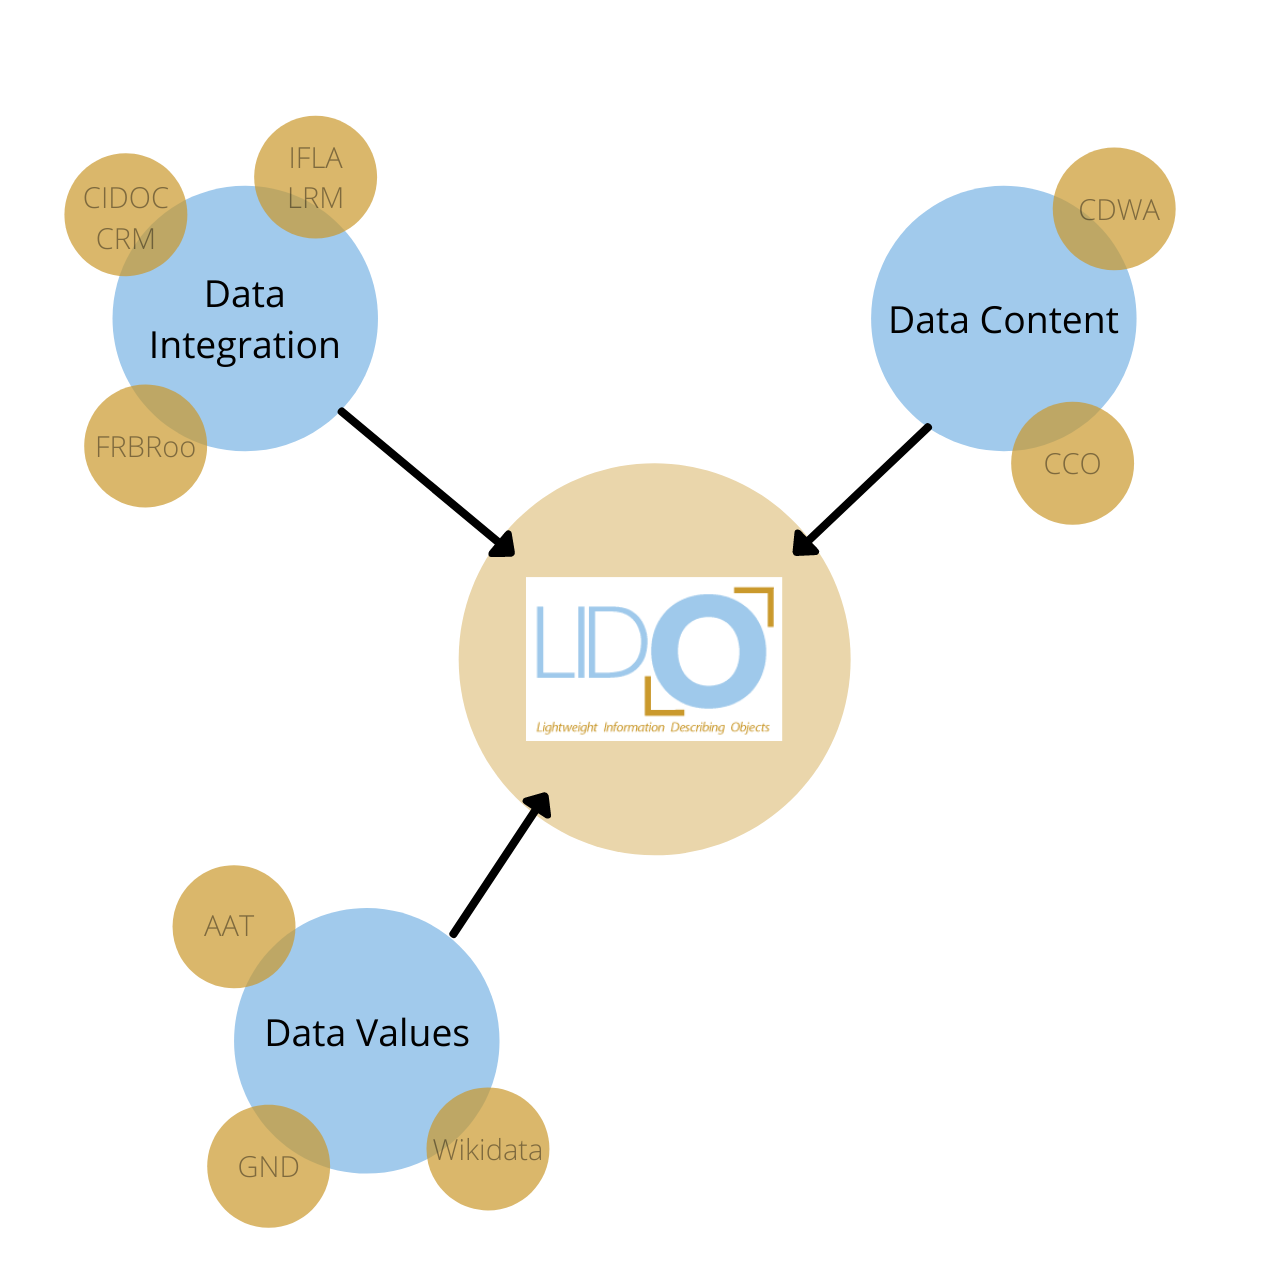
\includegraphics[width=\textwidth]{medias/figure_related-standards.png}}
	\caption{Standards liés au LIDO} 
\end{figure} \newline

Le modèle LIDO a été conçu selon les considérations suivantes :

\begin{itemize}
    \item Réutiliser les normes existantes : Les modèles préexistants de représentation des métadonnées du patrimoine culturel contiennent des propositions qui sont encore valables aujourd'hui. L'ojectif  a été de les réutiliser dans la conception de la LIDO. 
    \item Utiliser des technologies éprouvées : Les métadonnées doivent être traitées dans un large éventail d'environnements système. Le choix de technologies propriétaires ou mal supportées peut entraîner des obstacles et des coûts inutiles.
    \item Faciliter l'interopérabilité  :Les métadonnées sont déplacées, transformées, distribuées et interconnectées à un rythme croissant. Le LIDO devrait donc faciliter et encourager des niveaux d'harmonisation plus élevés que par le passé. Outre les considérations techniques et organisationnelles, les correspondances entre LIDO et les normes ainsi que les modèles d'autres domaines sont des outils essentiels pour permettre et maintenir une telle harmonisation.
    \item Permettre l'adaptabilité :Le paysage de l'information évolue en permanence, faisant apparaître de nouvelles exigences auxquelles il faut répondre sans invalider les enregistrements de données existants. Il faut donc prévoir des adaptation dans le cadre du modèle. En outre, les métadonnées du patrimoine culturel continueront d'être produites à des degrés divers de détail et de granularité. Le modèle doit donc pouvoir s'adapter à des descriptions d'objets d'une richesse très différente en permettant l'introduction de restrictions spécifiques à l'application.
\end{itemize} 
Le choix du XML a été fait en tenant compte tenu de la maturité de celui-ci et de son large soutien dans la sphère du traitement de l'information. Il est possible de penser que cette technologie est et restera une plate-forme solide et fiable pour le schéma de métadonnées du LIDO.\newline

Le langage XML lui-même définit le format des éléments de balisage (souvent appelés balises) et la manière dont ils peuvent être imbriqués pour former une structure arborescente. Tout document XML qui respecte la syntaxe de base des éléments et dont les balises de début et de fin correspondent est dit bien formé.

Pour avoir un traitement prévisible du contenu du document, l'ordre et l'occurrence des éléments de balisage sont généralement limités par un schéma (il s'agit des règle de grammaire du document). Il existe au moins trois langages (DTD, RELAX NG et XSD) permettant d'écrire des définitions de schéma XML. Le schéma LIDO est écrit dans le langage XML Schema Definition (XSD), qui peut être considéré comme le plus expressif de ces trois langages. \newline

La spécification de base du LIDO est définie dans un document XSD. Ce document de schéma peut être utilisé pour vérifier si un enregistrement LIDO est conforme à toutes les règles et restrictions indiquées dans le schéma. Cette validation est essentielle lorsque l'enregistrement LIDO doit être traité pour être utilisé dans des bases de données, des portails web ou dans des chaînes de transformation telles que celles utilisées dans les portails d'agrégation à grande échelle. \footcite{lido_primer}

\begin{figure}[h!]
	\centerline{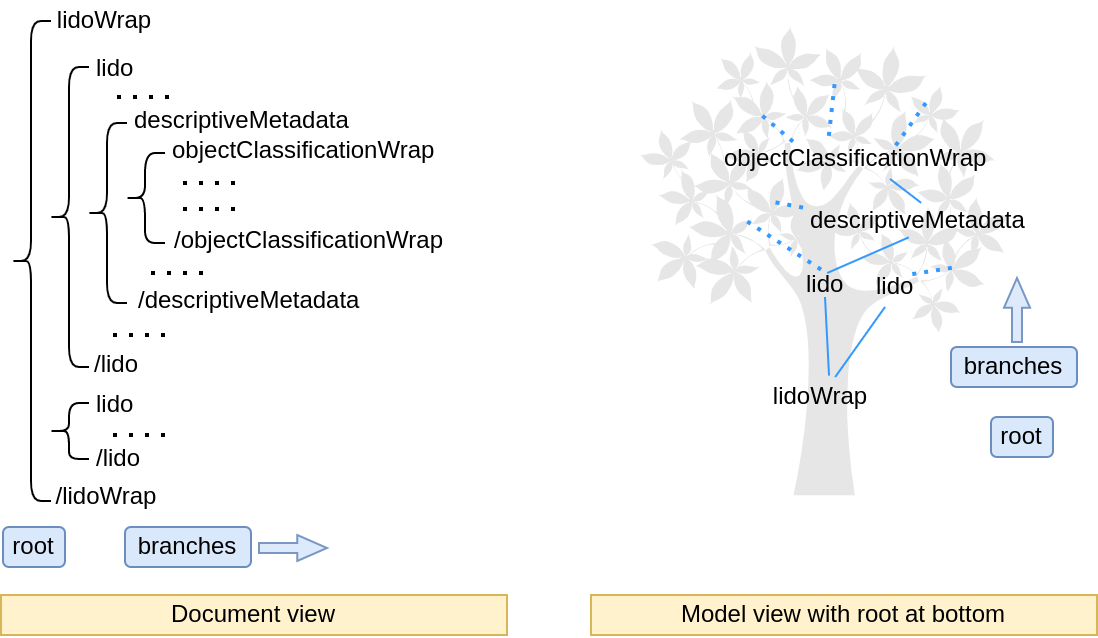
\includegraphics[width=\textwidth]{medias/figure_root-branches.png}}
	\caption{Structure de l'arborescence LIDO} 
\end{figure}
 \subsection{Pourquoi avoir choisi LIDO ?}

Tout d'abord, comme nous l'avons expliqué dans notre introdution, le moment était propice à la mise en place de la stratégie d'agrégation. La création d'un service du numérique au Ministère de la Culture, à permis d'établir une infrastructure commune et a donc mid en exergue le besoin d'uniformiser les flux de données pour industrialiser et massifier les quantités de données traitées par le ministère. Pour répondre a ce besoin c'est le LIDO qui est ressorti comme le modèle à utiliser.\newline

Il faut noter qu'il existait ben au ministère des formats d'échange de données culturelles: Le format d'export Joconde, le DC en OAI-PMH pour le moteur collection. mais ceux-ci étaient limités en termes de données, peu compatibles et ne proposaient aucun alignements vers d'autres standards.\newline

Le choix de LIDO comme standard de circulation pour l’agrégation des données muséales s’explique par plusieurs facteurs. Tout d’abord, LIDO est un modèle qui offre une interopérabilité élevée, ce qui est essentiel pour les musées qui souhaitent diffuser leurs collections à une échelle nationale ou internationale. En adoptant un modèle standardisé, les musées peuvent s’assurer que leurs données seront compatibles avec celles d’autres institutions, ce qui facilite l’agrégation et la diffusion des informations. \newline

Un autre avantage majeur de LIDO est sa simplicité. Contrairement à des modèles plus complexes comme CIDOC CRM, LIDO est basé sur le XML. Ce format est déjà utilisé dans de nombreux cas de figures, c'est le cas par exemple pour l'EAD en archives. Ce format est connu des archivistes et des documentalistes, ce qui pourrait le rendre plus ateignable pour des professionels des musées (même si c'est ne sont pas eux qui vont saisir les données en LIDO, ils pourront avoir une idée de la forme que l'export va prendre).\newline

LIDO est également un modèle conçu pour répondre aux besoins spécifiques des musées. Contrairement à d’autres standards plus génériques, LIDO prend en compte les spécificités des objets muséaux, en incluant des éléments comme les informations de provenance, les données contextuelles et les liens avec d’autres objets. Cela permet de capturer la complexité des collections muséales, tout en garantissant que ces informations peuvent être diffusées de manière standardisée. \newline

Un autre facteur qui a contribué au succès de LIDO est la gouvernance du modèle. Développé par l’ICOM et d’autres institutions culturelles internationales, LIDO bénéficie d’un soutien institutionnel fort, ce qui garantit la pérennité du modèle et sa capacité à évoluer pour répondre aux nouveaux défis du secteur culturel. En outre, LIDO est soutenu par une infrastructure technique solide, avec des outils et des ressources disponibles pour faciliter son adoption par les musées et les développeurs de systèmes de gestion de collections.

 \chapter{Notre proposition basée sur le modèle LIDO}
 \subsection{Les mappings, besoin de s'assurer que les données peuvent toutes
êtres portées par le modèles}

\textbf{Les Difficultés des Mappings entre Différents Modèles de Données : Dublin Core, RDF et LIDO }\newline

L’intégration de données hétérogènes dans des formats variés est un défi majeur dans la gestion des informations culturelles. Les institutions telles que les musées, les bibliothèques et les archives doivent souvent mapper ou convertir des données entre différents modèles de métadonnées.\newline

Le mapping, ou faire un mappage consiste à établir des correspondances entre différents modèles de données. On peut avoir besoin d’effectuer ce procédé lors d’une migration de données d’un système à un autre au sein d’une même institution. Dans notre cas, nous avons effectué cet exercice pour s’assurer que les données provenant des agrégateurs intermédiaires et des institutions partenaires du ministère, pouvaient bien être portées par le modèle LIDO. Pour faire cette vérification nous avons collecté et eu accès aux données telles qu’elles sont dans les bases de données des partenaires et nous les avons mappés pour voir comment elles pouvaient être intégrées dans le modèle LIDO. \newline

Comme nous l’avons expliqué précédemment, parmi les modèles utilisés par les partenaires, nous avons le  Dublin Core (DC), et les données exprimées en RDF (Resource Description Framework) ainsi que le format de l’export Joconde, et des formats propres à un agrégateur ou une institution.
Ces standards, présentent des divergences notables lorsqu'il s'agit de les aligner avec le LIDO. Les difficultés rencontrées lors du mappage entre ces modèles se situent à plusieurs niveaux : la sémantique, la granularité, la structure des données, et l'harmonisation des 
vocabulaires. Pour mieux comprendre ces défis, il est essentiel d’illustrer ces difficultés à travers des exemples concrets.
Les plus grandes difficultés que nous avons rencontré sont survenues ont été lors du mappage entre Dublin Core et LIDO, ou entre RDF et LIDO. Ces difficultés résident dans la disparité des concepts sémantiques. Chaque modèle a été conçu avec des objectifs spécifiques et des interprétations sémantiques propres. \newline

Prenons le concept de "contributeur". Dans Dublin Core, le terme "creator" fait référence à toute personne ou entité ayant participé à la création ou à l'élaboration d'une ressource. Cependant, cette définition est volontairement large pour s'adapter à différents types de ressources (livres, articles, pages web, etc.).\newline

Dans LIDO, le terme "créateur" est plus précisément subdivisé. Par exemple, un contributeur à une exposition d'art peut être catégorisé comme "peintre", "auteur", ou "photographe". Le modèle LIDO introduit une granularité plus fine avec des distinctions entre différents types de participants, chacun associé à un rôle précis dans la chaîne de production d’un objet culturel. En effet, le modèle Lido est composé d'éléments et d’attributs. Pour le créateur d’une peinture on modélise un événement de création de l'œuvre, dans lequel on intègre un élément “acteur” qui a pour attribut “créateur”, ou même “peintre” sur on veut être plus précis. 

\begin{figure}[h!]
	\centerline{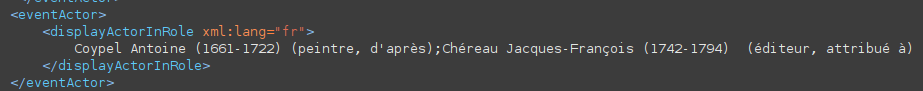
\includegraphics[width=\textwidth]{medias/figure_actor_2.png}}
	\caption{Exemple d'un peintre modélisé en LIDO}
\end{figure}
\begin{figure}[h!]
	\centerline{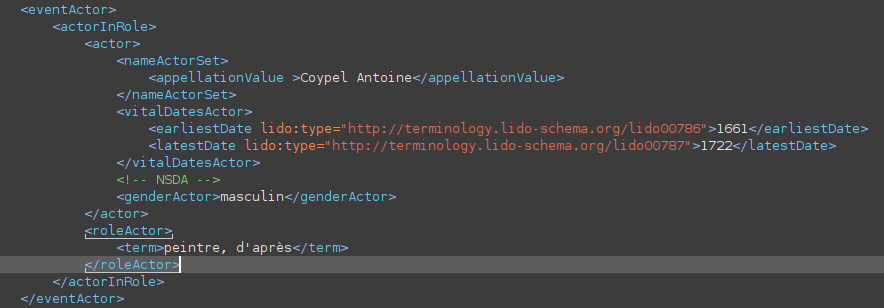
\includegraphics[width=\textwidth]{medias/figure_actor.png}}
	\caption{Exemple développé d'un peintre modélisé en LIDO}
\end{figure}

Lors du mappage, cette différence sémantique peut poser problème. Un contributeur générique dans Dublin Core doit être associé à un rôle spécifique dans LIDO. Si le rôle n'est pas précisé dans la source Dublin Core, il devient difficile de déterminer quelle sous-catégorie utiliser dans LIDO. Cette ambiguïté peut entraîner des erreurs de mappage ou la perte de détails importants.\newline

Dans le cas de RDF, les relations sont souvent exprimées de manière implicite à travers des triplets (sujet-prédicat-objet). Par exemple, une relation comme "Personne A a contribué à l'œuvre B" peut être définie de manière flexible, ce qui rend l’expression des rôles plus souple mais aussi moins spécifique. Pour adapter cette relation dans un cadre comme LIDO, il faudrait créer une correspondance précise, définissant le type de contribution en fonction des catégories disponibles dans LIDO.\newline

\textbf{Problèmes de Granularité}\newline

La granularité des données varie considérablement entre ces modèles, et cela devient particulièrement évident lors du mappage de données d'un modèle à un autre.\newline

Dans Dublin Core, l’élément "Date" est souvent utilisé pour désigner une date associée à la ressource. Cela peut inclure la date de création, la date de modification, ou la date de publication, mais le modèle ne fait pas de distinction claire entre ces différentes possibilités. Un document d'archive numérisé, par exemple, peut simplement avoir une seule date associée dans Dublin Core sans préciser s'il s'agit de la date de création ou d'une autre.\newline

En revanche, LIDO dispose de plusieurs éléments distincts pour capturer différentes dates liées à l’objet culturel, comme la "date de production", la "date d'acquisition", ou encore la "date d’exposition". Effet  cChaque date doit être associée à un événement, que ce soit un événement de création, d'acquisition, de découverte, etc…. Si on mappe des données de Dublin Core vers LIDO, la simple information de date ne suffit pas : il faut déterminer quelle catégorie de date correspond à celle fournie par Dublin Core, sinon on risque de perdre l’information..
Ce problème de granularité apparaît également lors du mappage de données RDF vers LIDO. Dans un graphe RDF, la date peut être liée à plusieurs entités ou événements par des relations spécifiques, mais ces relations ne correspondent pas toujours directement aux catégories de dates dans LIDO. Cela nécessite une analyse minutieuse du contexte RDF pour éviter une perte de précision lors du mappage. \newline

\textbf{Différences Structurelles}\newline

Les modèles de données Dublin Core, LIDO et RDF adoptent des structures très différentes, ce qui complique leur alignement.\newline

Dublin Core suit une structure relativement plate, avec des éléments de métadonnées tels que "titre", "créateur", "contributeur", et "sujet" placés au même niveau hiérarchique. Dans ce modèle, il n'y a pas de relation hiérarchique complexe entre ces éléments, et chaque élément se rapporte directement à la ressource décrite. Par exemple, une œuvre d’art dans Dublin Core pourrait être représentée avec un titre ("La Joconde"), un créateur ("Léonard de Vinci"), et une description simple.\newline

En revanche, LIDO utilise une structure hiérarchique plus complexe pour représenter les objets et leurs relations avec d'autres entités. Par exemple, une œuvre d’art serait décrite dans LIDO avec des sections distinctes pour le "titre", le "créateur", mais aussi pour des événements spécifiques comme l’acquisition, l’exposition, ou les restaurations. Ces événements sont eux-mêmes subdivisés avec des détails supplémentaires, tels que la date de l’événement, le lieu, et les participants. LIDO suit la structure en arborescence qui est commune aux modèles en XML.\newline

Le passage d’un modèle de structure plate (Dublin Core) à un modèle de structure structuré et hiérarchique (LIDO) nécessite souvent une réorganisation complète des données. Il faut non seulement redistribuer les éléments, mais aussi les relier de manière à respecter la hiérarchie de LIDO, sans pour autant perdre la qualité de la donnée. \newline

Dans RDF, les données sont souvent exprimées sous forme de graphes, où les relations sont définies comme des triplets entre des ressources. Si cette flexibilité est utile pour exprimer des relations complexes, elle nécessite une reformulation dans des systèmes comme LIDO, où les données doivent être présentées dans une structure hiérarchique. Par exemple, une relation RDF simple comme "Léonard de Vinci a peint la Joconde" peut devoir être traduite dans une structure LIDO où "Léonard de Vinci" serait placé dans une section distincte dédiée à l'événement de création de la Joconde, avec des métadonnées supplémentaires sur son rôle exact dans le processus créatif.\newline

Un autre défi crucial dans le processus de mappage est l'harmonisation des vocabulaires utilisés dans les différents modèles.\newline

Dans Dublin Core, les termes sont souvent choisis par l’utilisateur, avec peu d'obligation d'utiliser des vocabulaires contrôlés. Par exemple, pour l'élément "type", un utilisateur peut choisir d’indiquer simplement "peinture", tandis qu’un autre pourrait spécifier "huile sur toile". Ces deux entrées font référence à la même chose, mais ne sont pas normalisées.\newline

En revanche, LIDO dépend de vocabulaires contrôlés et de listes normatives pour assurer la cohérence et l'interopérabilité entre les institutions. Par exemple, une institution pourra choisir des termes précis provenant de thesaurus comme l’Art \& Architecture Thesaurus (AAT) pour décrire un objet et s'aligner sur ces thésaurus communs. \newline

Dans le cas de RDF, les vocabulaires peuvent également varier en fonction des données liées. Par exemple, une œuvre pourrait être associée à plusieurs schémas de classification RDF différents, chacun ayant sa propre ontologie. Lors du mappage vers LIDO, il faut non seulement traduire les termes RDF, mais aussi s'assurer qu'ils correspondent aux vocabulaires contrôlés utilisés dans le cadre LIDO, ce qui peut nécessiter l'utilisation d'outils de normalisation ou de ponts sémantiques. \newline

 \subsection{L’importance de documenter un modèle de données}

Dans le domaine de la gestion de l'information, la documentation d’un modèle de données joue un rôle fondamental pour garantir la clarté, l'accessibilité et la pérennité des données. Une documentation bien structurée et accompagnée d'exemples contextualisés, permet non seulement de rendre les données compréhensibles, mais elle facilite également leur réutilisation et leur intégration dans divers systèmes. Cette importance est particulièrement manifeste dans les institutions culturelles et archivistiques, où la gestion de métadonnées complexes exige une documentation rigoureuse. Dans notre cas, nous avons eu besoin de traduire la documentation du modèle LIDO, déjà existante, pour donner accès à l’information en français. Mais nous ne nous sommes pas arrêtés à la traduction, nous avons adapté la documentation pour l’alimenter des divers exemples rencontrés lors de la production des mappings. \newline

\textbf{Pérennité et traçabilité des données}\newline

Un des rôles principaux de la documentation est de garantir la pérennité des données dans le temps. Les données archivistiques, par exemple, ne se limitent pas à des documents statiques, elles sont dynamiques et évoluent constamment en fonction des nouvelles acquisitions, des mises à jour ou des recherches scientifiques. C'est également vrai pour des collections de muséesn même si la description physique de l'ojbet ne va probablement pas changer, des informations sur ses origines et son histoire peuvent émerger (la recherche de provenance prends de plus d'importance dans la gestion des collections). Des données liées aux mouvements de l'objets peuvent aussi être ajoutées (sa présence dans une exposition, son déplacement vers une autre institution, etc...). \newline

Sans une documentation claire, il devient difficile de gérer les changements et d'assurer une traçabilité de l'information. Cela est particulièrement vrai pour les Archives nationales françaises, qui ont adopté des systèmes modernes comme Records in Contexts (RiC), un modèle qui permet de mieux contextualiser les données archivistiques en fonction des relations entre entités.\footcite{clavaud} \newline

En prenant l'exemple des archives, on doit noter qu'elles doivent être continuellement enrichies pour améliorer la qualité et l’exploitabilité des métadonnées. Cela nécessite de s'appuyer sur une documentation structurée qui permet de retracer l’historique des changements et des mises à jour effectuées. \newline

\textbf{Accessibilité et partage des données}\newline

Une autre raison cruciale de bien documenter un modèle de données est d'assurer l'accessibilité des informations, non seulement pour les experts techniques mais aussi pour d’autres utilisateurs comme les chercheurs ou les administrateurs. Une documentation bien rédigée agit comme une feuille de route qui guide les utilisateurs à travers les complexités des données et des relations entre elles.\newline

Par exemple, dans le contexte de la gestion des données ouvertes, la documentation devient essentielle pour permettre aux différentes parties prenantes (institutions, chercheurs, développeurs) d'accéder et de manipuler les données. Comme indiqué dans l’article de Florence Clavaud,  le partage de données entre institutions nécessite une structure de documentation solide qui facilite l’accès et garantit une utilisation correcte des informations. \footcite{clavaud}\newline, 

Au sein des Archives nationales, les chercheurs qui consultent des collections spécifiques dépendent également d’une documentation claire pour comprendre comment les archives sont structurées, classées et liées à des entités ou événements. Sans une documentation appropriée, l’accès aux informations archivées devient complexe, voire impossible. Cela peut affecter la recherche et même conduire à des erreurs dans l’interprétation des données.\newline

\textbf{Interopérabilité entre systèmes et institutions}\newline

L'interopérabilité des données entre différents systèmes et institutions repose sur la capacité à partager des informations dans des formats compatibles. Une documentation claire est essentielle pour garantir que les différents acteurs qui manipulent les données puissent utiliser des normes communes et interpréter correctement les modèles de données. Par exemple, l'intégration des métadonnées archivistiques dans des portails comme Europeana ou Archives Portal Europe nécessite l’utilisation de normes internationales comme EAD (Encoded Archival Description) et EAC-CPF (Encoded Archival Context – Corporate bodies, Persons, and Families).\newline

Le modèle LIDO-MC a vocation à structurer les flux entre les institutions et le ministère. La documentation que nous proposereons devra être officielle, validée, à la fois compréhensible au plus grand nombre dans son but, et techniquement plus complexe pour permettre des développements de connecteurs par les éditeurs logiciels de gestion des collections. \newline

\textbf{Les difficultés rencontrées lors de la documentation d’un modèle de données}\newline
Bien que la documentation d’un modèle de données soit essentielle, ce processus présente plusieurs défis qui peuvent rendre la tâche complexe.
\begin{itemize}
    \item La complexité technique des modèles
Les systèmes d'information modernes sont souvent complexes, avec des modèles de données qui incluent plusieurs entités, relations et types de données. Documenter ces modèles nécessite une compréhension approfondie de la structure des données et de leur interaction. 
    \item. Maintien de la cohérence lors de l'évolution des systèmes
Un autre défi majeur est le maintien de la cohérence entre les différentes versions d’un modèle de données à mesure que les systèmes évoluent. Parfois, les données doivent être migrées d'un système à un autre ou enrichies pour répondre à de nouveaux besoins. Cela peut entraîner des incohérences si la documentation n'est pas mise à jour correctement. 
Les Archives nationales françaises ont, par exemple, connu des difficultés lors de la mise à jour de leur système d’information archivistique (SIA) pour intégrer la plateforme d’archivage électronique ADAMANT.\footcite{clavaud} La documentation des processus et des relations entre les différentes entités était essentielle pour garantir que ces modifications n'introduisent pas d'erreurs ou de pertes d'information.
    \item La diversité des utilisateurs et des besoins
Documenter un modèle de données peut également être compliqué en raison de la diversité des utilisateurs. Alors que certains utilisateurs, comme les développeurs, ont besoin d'une documentation technique détaillée, d'autres, comme les chercheurs ou le grand public, nécessitent une documentation plus accessible et compréhensible. Trouver un équilibre entre ces différents niveaux de détail peut être difficile et demande une planification minutieuse.
Selon les principes de la gouvernance des données ouvertes, la documentation doit être 
suffisamment flexible pour répondre aux besoins des experts techniques tout en restant accessible aux non-spécialistes. Cela signifie que la documentation doit souvent être organisée en plusieurs couches, avec des détails techniques plus approfondis pour les développeurs et des explications plus simples pour les utilisateurs non techniques.

\end{itemize}

\textbf{À qui s’adresse la documentation d’un modèle de données?}\newline

La documentation d'un modèle de données s'adresse à plusieurs types d’utilisateurs, chacun ayant des besoins spécifiques en termes de détails et d'accessibilité.\newline

Les développeurs et les administrateurs de systèmes sont les principaux utilisateurs de la documentation technique. Ils ont besoin d'une compréhension détaillée de la structure des données et des relations entre les entités pour configurer, maintenir et optimiser les bases de données. Sans une documentation adéquate, ils risquent de commettre des erreurs dans la gestion des données ou de ne pas être en mesure de résoudre rapidement les problèmes qui surviennent. Ces développeurs ne sont généralement pas du personnel aux institutions, ils travaillent pour des éditeurs de logiciels. En effet, les institutions culturelles font évoluer leurs outils de plus en plus vers des outils "sur étagère" que vers des solutions développées spécifiquement. Elles préfèrent une relation commerciale classique à devoir maintenir des compétences techniques en leur sein, et devoir gérer l'obsolescence d'outils créés par strates de fonctionnalités. Donc les éditeurs sont les principaux destinataire de cette documentation.\newline

Les archivistes et chercheurs, qui utilisent les systèmes d’information pour accéder aux données archivistiques, dépendent également de la documentation. Une documentation claire leur permet de comprendre comment les données sont organisées, classées et liées entre elles. Cela leur permet non seulement d’accéder rapidement aux informations nécessaires, mais aussi de les interpréter correctement dans leurs recherches. \newline

Enfin, dans le cadre de la donnée ouverte, le grand public peut également être un utilisateur des systèmes d’information. Pour ces utilisateurs, la documentation doit être simplifiée et accessible afin de leur permettre de naviguer dans les systèmes et d'accéder aux informations sans avoir besoin d'une expertise technique avancée. Dans le domaine de la culture et des archives, l’accès du grand public aux données est souvent encouragé pour démocratiser l'information, et cela nécessite une documentation claire et concise.\newline

La documentation d’un modèle de données est une étape essentielle pour assurer la clarté, l’accessibilité et la pérennité des systèmes d’information. Elle permet de structurer les données, de garantir leur traçabilité, d’améliorer leur interopérabilité, et de faciliter leur gestion et leur partage. Cependant, ce processus présente plusieurs défis, notamment le aprocessus d’évolution des systèmes et la complexité technique des modèles. Ces défis peuvent être surmontés avec une planification rigoureuse et une mise à jour constante de la documentation. Enfin, il est essentiel que cette documentation soit adaptée aux différents publics qui l’utiliseront, qu’il s’agisse des développeurs, des chercheurs ou du grand public, afin de garantir une utilisation optimale des données et une interopérabilité entre systèmes.\newline

\textbf{Le profil d’application LIDO-MC}\newline

Un avantage du modèle LIDO est la possibilité de créer un profil d'application qui 
Un profil d’application LIDO peut contenir des éléments de restrictions, ou commander/imposer des vocabulaires spécifiques, et plus encore.
Un profil d’application est toujours un « sous-standard » de son parent. Il peut préciser la sémantique d’un élément par rapport au LIDO générique, mais il ne change jamais la sémantique de cet élément.
De plus, les éléments et attributs obligatoires ne doivent pas être déclarés facultatifs. Cela garantit qu’un enregistrement LIDO conforme à un profil d'application reste aussi conforme au standard LIDO générique.\newline

Les règles d’un profil d’application peuvent être exprimées, soit dans un document texte (html,etc…), soit par un ensemble de règles exploitables par une machine (XML Schema, Schematron).
Idéalement le profil d’application contient les 2, il fournit une documentation qui explique les règles et le contexte, et il fournit aussi un fichier exploitable par une machine qui vérifie automatiquement la conformité du document.\newline

Lors de notre stge c'est ce que nous avont choisi de faire. Pour avoir à la fois le document avec la documentation lisible par un humain, et celle avec les règles exploitable par une machine, nous avons choisi de créer un ODD (One Document Does it all).(Voir annexe).
Le LIDO Application Profile Workflow, est la manière recommandée pour créer des profils d’application. Cette méthode fournit un moyen facile de documenter les différences entre le profil d'application et le LIDO générique, ainsi que de produire de la documentation et des règles xploitables par des machines pour le profil. \newline


Le workflow se construit autour d'un fichier XML ODD définissant le profil LIDO. Ce fichier contient toutes les informations que les utilisateurs doivent fournir pour que le processus produise un profil d'application LIDO valide : les métadonnées du profil, la documentation du profil et les règles du profil. De cette manière, la définition du profil sert de source unique pour les règles exploitables par la machine ainsi que pour la documentation HTML. Chacun des fichiers de sortie est produit par une seule transformation XSL de la définition de profil.
Ces règles sont  déclarées avec des règles Schematron. La documentation du profil dans la définition du profil suit TEI-Lite et est la source principale pour la documentation HTML. \newline

\begin{figure}[h!]
	\centerline{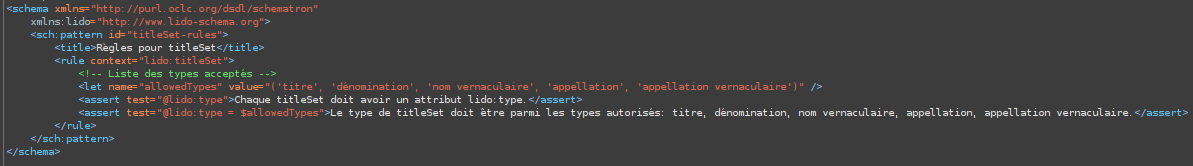
\includegraphics[width=\textwidth]{medias/exemple_schematron.png}}
	\caption{Exemple de la règle Schematron pour les TitleSet.}
\end{figure}

\begin{figure}[h!]
	\centerline{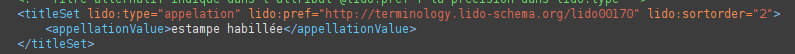
\includegraphics[width=\textwidth]{medias/exemple_attribut.png}}
	\caption{Exemple de l'usage de l'attribut autorisé.}
\end{figure}

Pour notre profil LIDO-MC, nous n'avons pas apporté de grands changemets dans les règles du LIDO générique. Ce que noous avons décidé de faire a été d'imposer une liste de termes à placer dans les attributs de certains éléments, pour qualifier des données de manière plus précise que si ont suivait les attributs propres au modèle. Ces termes peuvent notament servir à collecter des données qui ne sont pas nécessairement muséales, comme des livres, des manuscrits anciens, des films etc... Cette liste de termes a été constituée à partir des cas rencontrés lors de notre stage et est donc suceptible d'évoluer. \newline
\begin{figure}[h!]
	\centerline{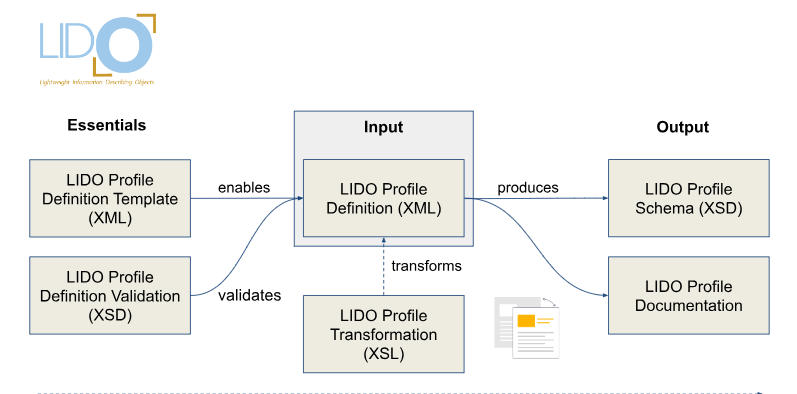
\includegraphics[width=\textwidth]{medias/Capture d’écran du 2024-09-15 07-21-40.png}}
	\caption{Workflow pour la création d'un profil d'application LIDO.\footcite{lido_primer}}
\end{figure}\newline


Notre objectif en proposant une documentation sous cette forme, est qu'elle réponde à un maximum des exigences mentionnées plus tôt, un document qui réuni toutes les informations et les règles de validation de manière structurée, devrait être suffusament adaptable pour des besoin de mis à jour. Ce document technique contient toutes les règles que les développeurs de logiciels ont besoin pour appliquer le modèle. De plus la documentation HTML produite est facilement lisible et accessible pour les autres utilisateurs. 



 \chapter{Les limites de nos propositions}
 \subsection{Les propositions qui sont faites ne sont pas toujours satisfaisantes.}


Comme évoqué précédemment, nous avons rencontré des difficultés lors du mapping d'un modèle vers le modèle. C'est en ayant conscience de ces difficultés que nous devons expliquer les limites du travail que nous avons proposé. \newline

Si, pour la plupart des modèles que nous avons analysés, nous avons pu trouver des correspondances satisfaisantes entre leurs données et la structure imposée par le modèle LIDO, ce n'a pas été le cas pour tous. \newline

Les données aux formats Dublin Core ne semblaient pas poser problème à première vue car elles n'étaient structurées que suivant les 15 éléments du modèle (parfois moins). Mais nous avons rapidement réalisé ces 15 éléments qui sont, à dessein, conçus pour être vagues afin de pouvoir porter tous les types de données utilisées par l'institution, n'étaient pas toujours utilisés de la même manière en fonction des institutions. \newline

Cette situation a donc rendu impossible la réalisation d'un mappage Dublin Core-LIDO, général. En effet, pour éviter de perdre la qualité des données fournies par toutes les institutions (pour les raisons évoquées plus tôt) il aurait fallu faire un mappage adapté à l'usage de Dublin Core que font chaque institution. Autant dire faire un mappage par institutions car elles en font toutes un usage légèrement différent… \newline

Faute de temps, nous n'avons pas été en mesure de fournir ce travail. Le mapping proposé pour les données en Dublin Core est donc obligatoirement insatisfaisant pour tous. Nous avons essayé de fournir un document qui soit général et représente les différents cas de figure et comment les faire correspondre dans le modèle LIDO, mais celui à forcément ses limites et ne pourra servir qu'à titre d'exemple, pas en temps qu’outil pour convertir les données.\newline

Pour revenir sur les difficultés rencontrées pour le mappage du modèle RDF utilisé pour les données du projet CapData Opéra vers le modèle LIDO, nous n'avons finalement pas proposé de mapping. Après plusieurs échanges avec Eudes Peyre et des tentatives de modélisation pour trouver des correspondances, nous nous sommes rendus compte que la tâche était trop complexe et que nous manquons de temps. Nous nous sommes donc accordés sur le fait que, pour s'assurer de conserver la qualité des données et toute leur complexité, il faudrait revenir sur ce chantier plus tard, peut-être une fois que la première version du modèle LIDO ministère de la Culture serait publiée. \newline

Nous avons également conscience que les mapping proposé pour les données de l’export Joconde n’est probablement pas parfait. Même si les correspondances entre les deux modèles ont pu être trouvées sans problème, d'autres ont demandé plus d'efforts et d'échanges avec nos interlocutrices au SMF. Il faut retenir que les propositions faites sont les notres, mais qu'une autre personnes pourraient en faire d'autres.\newline

Il en va de même pour la documentation. Notre approche a été celle e produire un document unique pour pouvoir centralsier l'information et donc pouvoir faciliter et tracer les mises jour. Cette documentation est conçue pour s'adresser à un public le plus large possible, mais une approche différente n'est pas forcément erronée.\newline

\textbf{les limites du modèle LIDO}. \newline

Le modèle LIDO est un modèle pour decrire les objets
musées, donc qui n’est pas toujours idéal pour décrire des objects différents, des évements et autres type de notices. Hors, durant notre stage, ce sont des cas de figure que nous avons rencontré, notament lors de nos échanges avec la ROF.\newline

Pour répondre aux besoins de l'agrégation le modèle de circulation LIDO sera adapté à la pluparts des données collectées, mais nous avons conscience que les métiers utilisent parfais des modèles plus adaptés à leur données qui sont difficilement convertible en LIDO.\newline

Pour répondre à un maximum de besoins et collecter des données en masse, il faudra des infrastructure capables de prendre d'autres formats

	%etc.
	
	
	\chapter*{Conclusion}
 La normalisation des données culturelles est devenue une nécessité incontournable dans le contexte actuel de la gestion du patrimoine culturel, où la numérisation et l'interopérabilité jouent un rôle central. \newline

Ce mémoire a mis en lumière les enjeux liés à la standardisation des données muséales, en particulier à travers le prisme du modèle LIDO (Lightweight Information Describing Objects). Ce processus, bien que complexe, est indispensable pour faciliter l'agrégation, l'exploitation et la diffusion des données dans un environnement numérique toujours plus interconnecté.\newline

La première partie de ce mémoire a exploré l'hisoire et les raisons pour lesquelles la normalisation des données culturelles est primordiale. L’un des défis majeurs auxquels font face les institutions culturelles, notamment les musées, est la diversité des formats de données. Ces derniers sont souvent développés en fonction des besoins spécifiques de chaque institution, ce qui engendre une fragmentation des pratiques et des données. Cette diversité freine l’interopérabilité des systèmes et rend difficile la circulation des informations entre les différentes plateformes locales, nationales et internationales.\newline

Dans ce contexte, la normalisation apparaît comme une solution essentielle pour transformer des données hétérogènes en un ensemble cohérent et homogène. En rendant les données comparables et interopérables, la normalisation facilite non seulement la recherche et la gestion des collections, mais permet aussi une meilleure visibilité de celles-ci. Elle offre ainsi aux musées et aux institutions culturelles une opportunité d’accroître leur rayonnement en rendant leurs collections accessibles à un public élargi via des plateformes en ligne comme la Plateforme Ouverte du Patrimoine (POP) en France, ou encore Europeana à l’échelle européenne.\newline

Le modèle de circulation LIDO se positionne comme un standard clé pour répondre aux besoins de l' agrégation des données muséales. Sa flexibilité et sa capacité à intégrer des données provenant de différentes sources en font un outil particulièrement adapté au contexte muséal, où les objets à décrire sont variés et complexes. LIDO permet non seulement de structurer les informations descriptives des objets, mais également d’assurer leur interopérabilité avec d’autres systèmes de gestion des collections.
Ce modèle se distingue par son format XML, facile à intégrer dans des bases de données existantes et compatible avec d’autres standards du web sémantique comme le RDF (Resource Description Framework). Cette compatibilité permet aux musées de publier leurs données sur des plateformes externes tout en garantissant une cohérence et une lisibilité des informations partagées. 

La normalisation des données, en plus de faciliter leur gestion, a un impact direct sur la valorisation du patrimoine culturel. En effet, en rendant les collections plus accessibles à travers des plateformes comme POP ou Europeana, les musées peuvent accroître leur visibilité à l’échelle nationale et internationale. Cette diffusion des collections ne profite pas seulement aux chercheurs et aux professionnels du patrimoine, mais également à un public plus large, intéressé par l’histoire, l’art ou la culture. \newline

L’agrégation des données permet de réunir des informations issues de multiples institutions et de les présenter de manière cohérente, offrant ainsi une meilleure expérience utilisateur. Le public peut accéder facilement à des collections jusqu'alors peu visibles, notamment celles des petits musées ou des institutions locales, qui bénéficient ainsi d'une meilleure visibilité. La réutilisation des données par des acteurs tiers (tourisme, éducation, recherche) ouvre également de nouvelles perspectives pour la valorisation du patrimoine culturel.
Perspectives d’évolution et d’amélioration.\newline

L’avenir de la normalisation des données culturelles repose en grande partie sur les évolutions technologiques. L’intelligence artificielle (IA) et le machine learning, en particulier, pourraient jouer un rôle crucial dans l’automatisation de certaines tâches liées à la normalisation et à l’interprétation des données. Ces technologies permettraient de faciliter la gestion des métadonnées en identifiant automatiquement des correspondances entre différents systèmes ou en enrichissant les descriptions des objets à partir de sources externes.\newline

La coopération internationale entre les institutions culturelles sera elle aussi essentielle pour harmoniser les pratiques à l’échelle mondiale. Des initiatives comme celles du CIDOC CRM ou d’Europeana montrent déjà des signes d’une volonté de convergence entre les différents acteurs du secteur culturel. \newline


Réflexion critique et recommandations
En conclusion, bien que des progrès significatifs aient été réalisés dans le domaine de la normalisation des données culturelles, de nombreux défis restent à relever. La standardisation des données, en particulier via des modèles comme LIDO, offre un potentiel considérable pour améliorer la gestion et la diffusion des collections. Cependant, il est crucial que ce processus soit accompagné d’un soutien aux institutions culturelles aux agrégateurs inermédiaires, notamment en termes de formation.\newline

Les professionnels du secteur devront continuer à s’adapter aux évolutions technologiques tout en maintenant un équilibre entre innovation et faisabilité. Les modèles de données comme LIDO offrent des solutions puissantes, mais ils doivent être ajustés aux besoins spécifiques des institutions, tout en garantissant une interopérabilité à l’échelle internationale. En ce sens, la normalisation ne doit pas être vue comme une fin en soi, mais comme un outil au service de la valorisation et de la préservation du patrimoine culturel.

        
	\addcontentsline{toc}{chapter}{Conclusion}
\newpage{\pagestyle{empty}\cleardoublepage}
	






%%%%%%%%%%%%%%%%%%

\appendix %Des appendices: tables figures, etc

\chapter[Documentation du modèle LIDO-MC]{Documentation du modèle LIDO-MC}
\begin{figure}[h!]
	\centerline{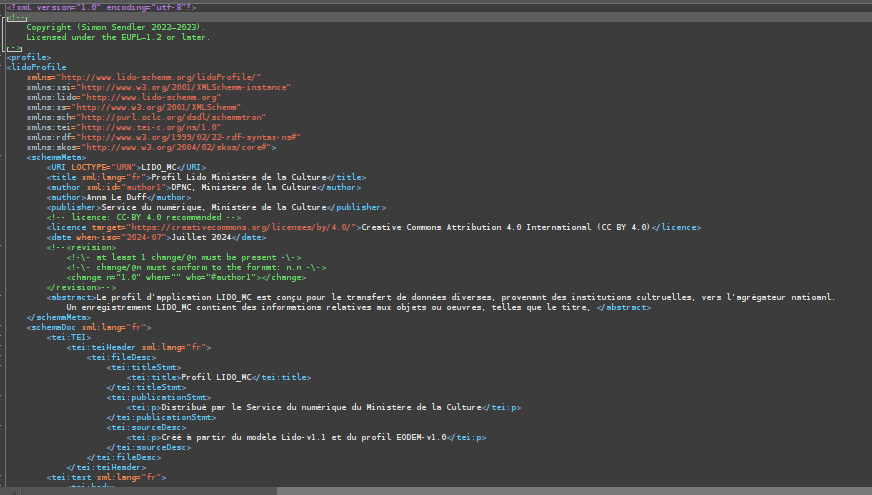
\includegraphics[width=\textwidth]{medias/extrait_ODD.png}}
	\caption{Extrait de l'ODD du modèle LIDO, Documetn complet à retrouver \href{https://github.com/annaleduff/Memoire_tnah_Anna_Le_Duff/tree/main/Annexes}{dans les annexes sur notre github}}
\end{figure}



\newpage{\pagestyle{empty}\cleardoublepage}

%%%%%%%%%%%%%%%%%%

\backmatter % glossaire, index, table des figures, table des matières.. (la bibliographie a déjà été appelée)

%\printindex

\printglossaries[title=Glossaire, style=long]
%\listoftables
%\listoffigures
\tableofcontents
\end{document}
